% concatenated from Permutation_sets_paper.tex
\documentclass[a4paper,12pt]{article}
\usepackage{hyperref}
\usepackage[T1]{fontenc}
\usepackage[utf8]{inputenc}

\usepackage[english]{babel}
\usepackage{mathtools}
\usepackage{amsfonts}
\usepackage{color}
\usepackage{amsmath}
\usepackage{amsthm}
\usepackage{amssymb}
\usepackage{mathrsfs}
\usepackage{amstext}
\usepackage{float}

\usepackage{todonotes}

\usepackage[normalem]{ulem}

\usepackage{graphicx}
\usepackage{tikz}
\usepackage{subfig}
\usepackage{pgfplots}
\usepgfplotslibrary{fillbetween}

%\usepackage[landscape]{geometry}
%\usepackage{lscape}

\usepackage{authblk}
\usepackage{stmaryrd}
\usepackage{makeidx}
\makeindex

\numberwithin{equation}{section}

%%%%%%%%%%%%% mit Numerierung %%%%%%%%%%%
\theoremstyle{definition}
\newtheorem{thm}{Theorem}[section]
\newtheorem{rem}[thm]{Remark}
\newtheorem{defi}[thm]{Definition}
\newtheorem{lem}[thm]{Lemma}
\newtheorem{cor}[thm]{Corollary}
\newtheorem{prop}[thm]{Proposition}
\newtheorem{ex}[thm]{Example}
\newtheorem{obs}[thm]{Observation}
\newtheorem{conj}[thm]{Conjecture}
\newtheorem{q}[thm]{Question}

%%% ohne Numerierung %%%%%%%%%%%%%%%%%%

\newtheorem*{thm*}{Theorem}
\newtheorem*{rem*}{Remark}
\newtheorem*{folg*}{Folgerung}
\newtheorem*{examples*}{Beispiele}
\newtheorem*{ex*}{Beispiel}
\newtheorem*{lem*}{Lemma}
\newtheorem*{prop*}{Proposition}
\newtheorem*{defi*}{Definition}
\newtheorem*{exercise*}{Übung}
\newtheorem*{conj*}{Conjecture}
\newtheorem*{q*}{Question}

\usepackage{cleveref}

% Bold
\newcommand{\bA}{\mathbf{A}}
\newcommand{\bB}{\mathbf{B}}
\newcommand{\bC}{\mathbf{C}}
\newcommand{\bD}{\mathbf{D}}
\newcommand{\bE}{\mathbf{E}}
\newcommand{\bF}{\mathbf{F}}
\newcommand{\bG}{\mathbf{G}}
\newcommand{\bH}{\mathbf{H}}
\newcommand{\bI}{\mathbf{I}}
\newcommand{\bJ}{\mathbf{J}}
\newcommand{\bK}{\mathbf{K}}
\newcommand{\bL}{\mathbf{L}}
\newcommand{\bM}{\mathbf{M}}
\newcommand{\bN}{\mathbf{N}}
\newcommand{\bO}{\mathbf{O}}
\newcommand{\bP}{\mathbf{P}}
\newcommand{\bQ}{\mathbf{Q}}
\newcommand{\bR}{\mathbf{R}}
\newcommand{\bS}{\mathbf{S}}
\newcommand{\bT}{\mathbf{T}}
\newcommand{\bU}{\mathbf{U}}
\newcommand{\bV}{\mathbf{V}}
\newcommand{\bW}{\mathbf{W}}
\newcommand{\bX}{\mathbf{X}}
\newcommand{\bY}{\mathbf{Y}}
\newcommand{\bZ}{\mathbf{Z}}

\newcommand{\ba}{\mathbf{a}}
\newcommand{\bd}{\mathbf{d}}
\newcommand{\be}{\mathbf{e}}
\newcommand{\boldf}{\mathbf{f}}
\newcommand{\bk}{\mathbf{k}}
\newcommand{\bm}{\mathbf{m}}
\newcommand{\bn}{\mathbf{n}}
\newcommand{\bu}{\mathbf{u}}
\newcommand{\bv}{\mathbf{v}}
\newcommand{\bw}{\mathbf{w}}
\newcommand{\bx}{\mathbf{x}}
\newcommand{\by}{\mathbf{y}}
\newcommand{\bz}{\mathbf{z}}

% Blackboard
\newcommand{\bbA}{\mathbb{A}}
\newcommand{\bbB}{\mathbb{B}}
\newcommand{\bbC}{\mathbb{C}}
\newcommand{\bbD}{\mathbb{D}}
\newcommand{\bbE}{\mathbb{E}}
\newcommand{\bbF}{\mathbb{F}}
\newcommand{\bbG}{\mathbb{G}}
\newcommand{\bbH}{\mathbb{H}}
\newcommand{\bbI}{\mathbb{I}}
\newcommand{\bbJ}{\mathbb{J}}
\newcommand{\bbK}{\mathbb{K}}
\newcommand{\bbL}{\mathbb{L}}
\newcommand{\bbM}{\mathbb{M}}
\newcommand{\bbN}{\mathbb{N}}
\newcommand{\bbO}{\mathbb{O}}
\newcommand{\bbP}{\mathbb{P}}
\newcommand{\bbQ}{\mathbb{Q}}
\newcommand{\bbR}{\mathbb{R}}
\newcommand{\bbS}{\mathbb{S}}
\newcommand{\bbT}{\mathbb{T}}
\newcommand{\bbU}{\mathbb{U}}
\newcommand{\bbV}{\mathbb{V}}
\newcommand{\bbW}{\mathbb{W}}
\newcommand{\bbX}{\mathbb{X}}
\newcommand{\bbY}{\mathbb{Y}}
\newcommand{\bbZ}{\mathbb{Z}}

% Calligarphic
\newcommand{\cA}{\mathcal{A}}
\newcommand{\cB}{\mathcal{B}}
\newcommand{\cC}{\mathcal{C}}
\newcommand{\cD}{\mathcal{D}}
\newcommand{\cE}{\mathcal{E}}
\newcommand{\cF}{\mathcal{F}}
\newcommand{\cG}{\mathcal{G}}
\newcommand{\cH}{\mathcal{H}}
\newcommand{\cI}{\mathcal{I}}
\newcommand{\cJ}{\mathcal{J}}
\newcommand{\cK}{\mathcal{K}}
\newcommand{\cL}{\mathcal{L}}
\newcommand{\cM}{\mathcal{M}}
\newcommand{\cN}{\mathcal{N}}
\newcommand{\cO}{\mathcal{O}}
\newcommand{\cP}{\mathcal{P}}
\newcommand{\cQ}{\mathcal{Q}}
\newcommand{\cR}{\mathcal{R}}
\newcommand{\cS}{\mathcal{S}}
\newcommand{\cT}{\mathcal{T}}
\newcommand{\cU}{\mathcal{U}}
\newcommand{\cV}{\mathcal{V}}
\newcommand{\cW}{\mathcal{W}}
\newcommand{\cX}{\mathcal{X}}
\newcommand{\cY}{\mathcal{Y}}
\newcommand{\cZ}{\mathcal{Z}}

% Sans Serif
\newcommand{\sfA}{\mathsf{A}}
\newcommand{\sfB}{\mathsf{B}}
\newcommand{\sfC}{\mathsf{C}}
\newcommand{\sfD}{\mathsf{D}}
\newcommand{\sfE}{\mathsf{E}}
\newcommand{\sfF}{\mathsf{F}}
\newcommand{\sfG}{\mathsf{G}}
\newcommand{\sfH}{\mathsf{H}}
\newcommand{\sfI}{\mathsf{I}}
\newcommand{\sfJ}{\mathsf{J}}
\newcommand{\sfK}{\mathsf{K}}
\newcommand{\sfL}{\mathsf{L}}
\newcommand{\sfM}{\mathsf{M}}
\newcommand{\sfN}{\mathsf{N}}
\newcommand{\sfO}{\mathsf{O}}
\newcommand{\sfP}{\mathsf{P}}
\newcommand{\sfQ}{\mathsf{Q}}
\newcommand{\sfR}{\mathsf{R}}
\newcommand{\sfS}{\mathsf{S}}
\newcommand{\sfT}{\mathsf{T}}
\newcommand{\sfU}{\mathsf{U}}
\newcommand{\sfV}{\mathsf{V}}
\newcommand{\sfW}{\mathsf{W}}
\newcommand{\sfX}{\mathsf{X}}
\newcommand{\sfY}{\mathsf{Y}}
\newcommand{\sfZ}{\mathsf{Z}}

% Fraktur
\newcommand{\fA}{\mathfrak{A}}
\newcommand{\fB}{\mathfrak{B}}
\newcommand{\fC}{\mathfrak{C}}
\newcommand{\fD}{\mathfrak{D}}
\newcommand{\fE}{\mathfrak{E}}
\newcommand{\fF}{\mathfrak{F}}
\newcommand{\fG}{\mathfrak{G}}
\newcommand{\fH}{\mathfrak{H}}
\newcommand{\fI}{\mathfrak{I}}
\newcommand{\fJ}{\mathfrak{J}}
\newcommand{\fK}{\mathfrak{K}}
\newcommand{\fL}{\mathfrak{L}}
\newcommand{\fM}{\mathfrak{M}}
\newcommand{\fN}{\mathfrak{N}}
\newcommand{\fO}{\mathfrak{O}}
\newcommand{\fP}{\mathfrak{P}}
\newcommand{\fQ}{\mathfrak{Q}}
\newcommand{\fR}{\mathfrak{R}}
\newcommand{\fS}{\mathfrak{S}}
\newcommand{\fT}{\mathfrak{T}}
\newcommand{\fU}{\mathfrak{U}}
\newcommand{\fV}{\mathfrak{V}}
\newcommand{\fW}{\mathfrak{W}}
\newcommand{\fX}{\mathfrak{X}}
\newcommand{\fY}{\mathfrak{Y}}
\newcommand{\fZ}{\mathfrak{Z}}

\newcommand{\frm}{\mathfrak{m}}
\newcommand{\frn}{\mathfrak{n}}
\newcommand{\frp}{\mathfrak{p}}

% Smybols
\newcommand{\elemcap}{\rotatebox[origin=c]{270}{$\in$}}
\newcommand{\elemcup}{\rotatebox[origin=c]{90}{$\in$}}
\newcommand{\es}{\emptyset}
\newcommand{\Gbar}{\overline{G}}
\newcommand{\la}{\leftarrow}
\newcommand{\longla}{\longleftarrow}
\newcommand{\La}{\Leftarrow}
\newcommand{\lra}{\leftrightarrow}
\newcommand{\Lra}{\Leftrightarrow}
\newcommand{\ra}{\rightarrow}
\newcommand{\longra}{\longrightarrow}
\newcommand{\Ra}{\Rightarrow}
\newcommand{\sm}{\setminus}
\newcommand{\sbse}{\subseteq}
\newcommand{\sbsn}{\subsetneq}
\newcommand{\spse}{\supseteq}
\newcommand{\spsn}{\supsetneq}
\newcommand{\tu}{\tilde{\cup}}

% Operators
\newcommand{\Argmin}{\operatorname{Argmin}}
\newcommand{\cl}{\operatorname{cl}}
\newcommand{\dv}{\operatorname{dv}}
\newcommand{\Fix}{\operatorname{Fix}}
\newcommand{\GF}{\operatorname{GF}}
\newcommand{\iu}{\mathrm{i}}
\newcommand{\id}{\operatorname{id}}
\newcommand{\Le}{L_2^{\text{extr}}}
\newcommand{\Lp}{L_2^{\text{per}}}
\newcommand{\Ls}{L_2^{\text{star}}}
\newcommand{\Max}{\operatorname{Max}}
\newcommand{\Min}{\operatorname{Min}}
\newcommand{\prob}{\operatorname{prob}}
\newcommand{\supp}{\operatorname{supp}}
\newcommand{\Var}{\operatorname{Var}}

% Commands
\newcommand{\CHECK}{\textcolor{red}{\textbf{CHECK}}}
\newcommand{\ol}{\overline}
\newcommand{\REF}{\textcolor{red}{\textbf{REFERENCE}}}
\newcommand{\T}{\tilde}
\newcommand{\TBC}{\textcolor{red}{\textbf{TO BE CONTINUED}}}
\newcommand{\TBD}{\textcolor{red}{\textbf{TO BE DONE}}}
\newcommand{\ul}{\underline}
\newcommand{\eps}{\varepsilon}
\newcommand{\epsi}{\epsilon}
\newcommand{\exT}{\epsi^{}_\cT}
\newcommand{\etp}{\eta^\text{p}_2}
\newcommand{\eoe}{\eta^\text{e}_1}
\newcommand{\ete}{\eta^\text{e}_2}
\newcommand{\dx}{\text{d}}
\newcommand{\ETe}{E^\text{extr}_\cT}
\newcommand{\ETp}{E^\text{per}_\cT}

\allowdisplaybreaks

\author{Dmitriy Bilyk, Nicolas Nagel, Ian Ruohoniemi}
%\affil{Chemnitz University of Technology \\ \texttt{nicolas.nagel@mathematik.tu-chemnitz.de}}
%\affil{\texttt{nicolas.nagel@mathematik.tu-chemnitz.de}}
%\affil{TU Chemnitz}
\title{Minimizing point configurations for tensor product energies on the torus}
%\title{Minimizers of  energies with tensor product structure on the torus}
\date{}

%\setlength{\parindent}{0pt}

\pgfplotsset{yticklabel style={text width=3em,align=right}}

\begin{document}
	
	\maketitle
	%\thispagestyle{empty}
	%\hspace{200pt}
	%\tableofcontents
	%\newpage
	%\thispagestyle{empty}
	%\mbox{}
	
	%\newpage
    
\begin{abstract}
 We study point configurations on the torus $\mathbb T^d$  that  minimize interaction energies with tensor product structure which arise naturally  in the context of discrepancy theory and  quasi-Monte Carlo integration. Permutation sets on $\mathbb T^2$  and Latin hypercube sets in higher dimensions (i.e. sets whose projections onto coordinate axes are equispaced points)  are natural candidates to be energy minimizers. We show that such point configurations that have only one distance in the vector sense minimize the energy for a wide range of potentials, in other words, such sets satisfy a tensor product version of universal optimality. This applies, in particular, to three- and five-point Fibonacci lattices. We also  characterize all lattices with this property and exhibit some non-lattice sets of this type.  In addition, we obtain several further structural results about global and local minimizers of tensor product energies. 
 
  %; a comprehensive list of such applications will be given in the appendix.%I don't think it's common to refer to specific sections in the abstract, so it might make sense to present this differently?
  %  This paper shows that under suitable but general assumptions, minimizing configurations must consist of points with distinct coordinates. Permutation sets in the two-dimensional torus and Latin hypercube sets in higher dimensions fulfill this separation property in an extreme way and thus form canonical candidates for (approximate) minimizers of tensor product energies. To this end we show%I think it's best to avoid using first person in formal writing although for this spot I'm not sure how to avoid it.
 %   that certain lattices in arbitrary dimensions with a particularly regular structure are global minimizers for a certain class of potentials. We also look at some other specific point configurations in the two-dimensional torus that are not captured by these lattices and investigate their optimality. We conclude with a particular property of permutation sets, relating two notions of $L_2$-discrepancy for these point sets, which also gives us a procedure of finding good candidates for minimizers algorithmically.
\end{abstract}

\section{Introduction}

\subsection{Energies with product structure}

Denote by $\bbT = \bbR/\bbZ$ the unit  torus, where we will identify elements in $\bbT$ with those in the half-open interval $[0, 1)$. In the present paper we explore the properties of minimizers of  interaction energies on $\mathbb T^d$ with kernels that have tensor product structure.  To be more precise, consider the kernel  $F: \mathbb T^d  \rightarrow [0, \infty)$ of the form 
\begin{equation}\label{e.f}
F(t_1, \dots, t_d)  = f(t_1) \dots f(t_d), 
\end{equation}
where %$G: \mathbb T^2 \rightarrow \mathbb R$ and 
$f: \bbT \ra [0, \infty)$. Throughout the paper we will assume that $f$, viewed  as   a non-negative  $1$-periodic function on $\bbR$, is \emph{even and continuous} on $(0,1)$. In most situations $f$ will actually be assumed to be continuous on the whole real line, but some  results also apply when $f$ is singular at $0$ in the sense of $\lim_{t \ra 0}f(t) = + \infty$. We will refer to both $F$ and $f$ as \emph{potentials} throughout the paper.


For a (multi)set of $N$ points $X = \{ \bx^0, \bx^1, \dots, \bx^{N-1} \} \subset \mathbb T^d$ with components $\bx^k = (x^k_1, \dots, x^k_d)$, we define the \emph{tensor product energy} as 
\begin{equation}\label{e.energy}
E_F(X) % = E_F ( {\bf{x}}^0, \dots, {\bf{x}}^{N-1} ) 
= \sum_{\substack{k, \ell=0 \\ k \neq \ell}}^{N-1}F({\bf{x}}^k -  {\bf{x}}^\ell) = \sum_{\substack{k, \ell=0 \\ k \neq \ell}}^{N-1} \prod_{i=1}^d  f(x_i^k - x_i^\ell).
\end{equation}
%where we denote ${\bf{p}}_i = (x_i, y_i)$.
This quantity can be intuitively viewed as the total potential energy of $N$ particles in positions ${\bf x}^0, \bx^1, \dots, {\bf x}^{N-1} $ which interact according to the potential given by $F$. One is then naturally interested in minimizing the energy \eqref{e.energy} over all $N$-point configurations and finding minimizing configurations of points, i.e.  equilibrium distributions. We shall call such configurations \emph{energy minimizers}. While extensive literature  exists on energy minimization in various domains in the case where the kernel $F({\bf{x}}, {\bf{y}})$ depends on the Euclidean (or another) distance between ${\bf{x}}$ and  ${\bf{y}}$ (see for example the book \cite{BHS}), kernels with tensor product structures have not received the same attention \cite{HO16, Nag25b}. %They've still received some attention though so it might be good to cite some papers here that do cover them.

%Denoting points ${\bf{p}}_i$ in the two-dimensional torus $\mathbb T^2 \simeq [0,1)^2$ % \simeq \mathbb S^1 \times S^1$ 
%as ${\bf{p}}_i = (x_i, y_i)$, we shall consider kernels of the form 
The condition that $f$ is even, or equivalently $f(t) = f (1-t)$, means that $f (x - y)$ depends only on the \emph{geodesic distance}
\begin{align} \label{eq:geod_dist}
    \delta(x, y) = \min\{|x-y|, 1-|x-y|\}
\end{align}
between $x$ and $y$ in $\mathbb T$. %This means that our kernel's behavior is determined by $f$'s behavior on $[0,1/2)$. 
For most potentials of interest, $f$ is decreasing on $(0,1/2]$, as this corresponds to the interaction being repulsive in each coordinate. 

 We remark that  the energy  \eqref{e.energy} of a configuration is invariant under symmetries of the torus (translations, reflections, and permutations of coordinates) and all uniqueness statements, e.g. in Definition \ref{def:perm_set} or Theorem \ref{thm:unique_dist_lat}, are to be understood modulo these symmetries.  In particular, since  the energy \eqref{e.energy} is translation invariant, we may assume without loss of generality  that ${\bf x}^0 = (0, \dots, 0)$.

Energies of the type \eqref{e.energy} with tensor product kernels \eqref{e.f} naturally arise in several fields such as discrepancy theory and quasi-Monte Carlo (QMC) integration. Warnock's formula \cite{HKP21, HO16, War72} states that minimizing the periodic $L^2$-discrepancy of $N$ points in $\mathbb T^d$ is equivalent to minimizing the  energy \eqref{e.energy} with the kernel \eqref{e.f}, where $f(t) = \frac12 - t + t^2$ on $[0,1)$. It is also known \cite{HO16, Nag25b}  that minimizing the worst-case integration error of the quasi-Monte Carlo rule over a certain Sobolev space corresponds to the energy minimization problem with the potential
\begin{align} \label{eq:qmc_potential}
    f_p(t) = 1 + \frac{p}{2} \left( \frac16 - t + t^2\right),
\end{align}
where $p > 0$ is a fixed parameter (notice that $f_6= 3f$, where $f$ is the aforementioned potential from Warnock's formula). Similar statements hold for other reproducing kernel Hilbert spaces (see the Appendix §\ref{s.potentials} and \cite{BD09, BT03} or \cite[§9]{NW10}). %While in the present paper we are mainly focused on the two-dimensional case, the aforementioned relations hold in all dimensions. 
The relation to discrepancy theory provides possible candidates for  energy minimizers, namely low-discrepancy sets. %"so-called" runs the risk of sounding a little pejorative.


\subsection{Dimension $d=2$: Permutation sets and Fibonacci lattices} 

Some of the most well-known low-discrepancy point sets in $\bbT^2$ include the digit-reversing \emph{van der Corput sets} when $N = 2^n$  (see e.g. \cite{HKP21} for a definition) and the \emph{Fibonacci lattices} which  will keep appearing in  this paper: if $N = F_j$ is a Fibonacci number, the $N$-point Fibonacci lattice is defined by
\begin{align} \label{eq:fib_lat}
	\Phi_j \coloneqq \left\{\left(\frac{k}{F_j}, \left\{\frac{k F_{j-1}}{F_j}\right\}\right): k=0, 1, \dots, F_j-1\right\},
\end{align}
where $\{\cdot\}$ denotes the fractional part.  This set can be thought of as a rational approximation to the famous Kronecker set $\big\{  (k/N, \{ k \varphi \} ): k \in \bbN_0 \big\}$, where $\varphi$ is the golden section. Fibonacci lattices have been studied extensively in the context of discrepancy theory and numerical integration and perform strongly in these settings \cite{BTY12-2, BTY12-1}.

Both of the aforementioned examples, the van der Corput set and the Fibonacci lattice, have important structural properties. First, these are $N$-point configurations that are subsets of the $(N\times N)$-grid
$$
\left\{ \left( \frac{k}{N}, \frac{\ell}{N} \right): \, k, \ell = 0,1,\dots, N-1 \right\}
$$
in $ [0,1)^2 \simeq \mathbb T^2$. We shall call such sets  {\it grid sets}. More importantly these examples are of the form 
\begin{equation}\label{e.permutation}
X_\sigma = \{ {\bf x}^k \}_{k=0}^{N-1} = \left\{\left(\frac{k}{N}, \frac{\sigma (k) }{N}\right): k=0, 1, \dots, N-1\right\},
\end{equation}
where $\sigma$ is a permutation of the set $\{0,1,\dots, N-1\}$  (if we assume ${\bf x}^0 = (0,0)$, that is we fix $\sigma (0) = 0$, we can view $\sigma $ just as easily as a permutation of $\{ 1,\dots, N-1\}$).

\begin{defi}\label{def:perm_set}
We shall call configurations $X \subset \mathbb T^2$ which (up to translations) have the form \eqref{e.permutation}  {\emph{permutation sets}}.  %The corresponding permutation $\sigma$ will be called the \emph{permutation type} of $X$.
\end{defi} 

A special place among the permutation sets is taken by  {\it integration lattices} (which we shall refer to simply as {\it lattices}), i.e. sets of the form 
\begin{equation}\label{e.lattice}
\left\{\left(\frac{k}{N}, \left\{\frac{hk }{N}\right\}\right): k=0, 1, \dots, N-1\right\},
\end{equation}
where $h$ and $N$ are relatively prime integers. The condition that $h$ and $N$ are relatively prime guarantees that \eqref{e.lattice} is indeed a permutation set. Notice that such sets are restrictions to $[0,1)^2$ of lattices in $\mathbb R^2$ generated by the vectors $(1/N, h/N)$ and $(0,1)$, which are $1$-periodic in both coordinate directions. Fibonacci lattices \eqref{eq:fib_lat} are particular examples of such sets.

We note that permutation sets are those sets whose projections onto both $x$- and $y$-axes are $N$ equispaced points, i.e. they are grid sets with exactly one point in each row and each column.  This interpretation suggests that, since many energies in dimension $d=1$ are minimized by equispaced points (see \S \ref{sec:equispaced}), it is natural to expect that permutation sets minimize tensor product energies on $\mathbb T^2$ for large classes of potentials. We then have the following question: {\emph{which conditions on the potential $f$ guarantee that  minimizers of the tensor product energy \eqref{e.energy} are permutation sets?}} This question admits a variety of versions and interpretations: e.g., when does this hold for all $N$, for specific values of $N$, or for all $N$ large enough? When are energies minimized by lattices? Does it hold if sets are restricted to the $(N\times N)$-grid? 

Based on the  particularly important role played by the Fibonacci lattices in low discrepancy constructions and on ample numerical evidence \cite{HO16}, we conjecture that whenever $N$ is a Fibonacci number,  \emph{the Fibonacci lattice minimizes the energy for a broad class of potentials $f$}. This conjectured phenomenon (the same configuration minimizing a large variety of energies) is a natural analogue of the notion of {\emph{universal optimality}}  that has been studied on the sphere $\mathbb S^d$ \cite{CK07} and in the plane \cite{CKMRV22}, and is known to be very rare. 





In the end, we remark that the condition that $f$ is logarithmically convex is very natural as it is necessary and sufficient for the tensor product $F$ to be convex as a function of $d$ variables \cite{SS12b}. 

\subsection{Higher dimensions $d\ge 3$} 
In dimensions $d \geq 3$ it becomes significantly harder to construct good point sets. To the knowledge of the authors, no study of global optimizers of $L_2$-discrepancy or quasi-Monte Carlo worst case errors in dimensions $d \geq 3$ has been carried out so far and only asymptotic results are known \cite{CS02, GSY16a}. A straightforward extension of the concept of permutation sets in higher dimensions to sets on the $N^d$-grid $\{k/N: k=0, 1, \dots, N-1\}^d$ leads to Latin (hyper)cubes.

\begin{defi} \label{def:lat_hypcube}
    A \emph{Latin hypercube set} is defined by permutations $\sigma_2, \dots, \sigma_d$ of the set $\{0, 1, \dots, N-1\}$ via
    $$
    X_{\sigma_2, \dots, \sigma_d} = \left\{\left(\frac{k}{N}, \frac{\sigma_2 (k) }{N}, \dots, \frac{\sigma_d(k)}N\right): k=0, 1, \dots, N-1\right\}.
    $$
\end{defi}
In other words, it is a set whose projections on all coordinate axes are equispaced points.  Thus a {\emph{permutation set}} is a Latin hypercube set with $d=2$. 
%\textcolor{red}{Note: Latin hypercube sets are precisely $(d-1, 1, d)$-nets in base $N$ living in the $N^d$-grid.}
Analogously to $\mathbb T^2$, lattices in $\bbT^d$ of the form 
$$\left\{\left(\frac{k}{N}, \left\{ \frac{h_2 k }{N}\right\} , \dots, \left\{ \frac{h_{d} k}N \right\} \right): k=0, 1, \dots, N-1\right\},
 $$ which are generated by a vector
$
\left(\frac1N, \frac{h_2}N, \dots, \frac{h_d}N\right)
$
with  $\gcd(h_2, N) = \dots = \gcd(h_d, N) = 1$, are common examples of Latin hypercube sets. %(The other $d-1$ generators of the lattice are just  the coordinate vectors ${\bf e}_2, \dots, {\bf e}_d$, and we abuse terminology by omitting them.)  % \emph{digital nets} with regular generator matrices \cite{}) are common examples of Latin hypercube sets. 
%It is an active area of research to find good lattice constructions, in particular it is not known of they can achieve asymptotic optimality for $d \geq 3$. \textcolor{red}{Optimality with respect to what? References? Maybe remove this sentence?}

Just as in the case of permutation set in dimension $d=2$,  the  same questions naturally arise in dimension $d\ge 3$: {\emph{For which potentials $f$ do  Latin hypercubes  minimize the tensor product energy? Can one identify specific lattices or other Latin hypercube sets which minimize large classes of energies?}}  

\subsection{Main results}
Even though complete answers to the aforementioned questions appear to be out of reach for now, we provide a plethora of interesting results 
which open up a new direction in energy minimization. In particular, we prove the following:

\begin{itemize}
\item As a first indication that permutation  and Latin hypercube sets might naturally be minimizers of tensor product energies in all dimensions $d\ge 2$, we show that points in (local) minimizers cannot coincide in any coordinate provided that the potential $f$ generates sufficient repulsion at small scales (Theorem \ref{prop:coordinate_improvement}). 
\item  In Theorem \ref{thm:optimality}, which can be considered the main result of the paper, we prove that  in all dimensions $d\ge 2$ {\emph{Latin hypercube sets with a single distance vector}} (in other words, sets of maximal separation in which each interaction contributes the same amount to the energy) minimize the tensor product energy with potential $f$  whenever the energy with potential $g= \log f $ on $\mathbb T$ is minimized by equispaced points. Sufficient conditions for this property include the following:  

(a) $f$ is logarithmically convex and decreasing on $(0,1/2]$, or 

(b) $\log f(t)$ %\todo{consistency of variable $t$} 
is absolutely monotone with respect to $s = \cos (2\pi t)$.

(See \S\ref{sec:equispaced} for more details) 
\item We  exhibit many  sets in dimensions with a single distance vector in dimensions $d\ge 2$. In fact, in Theorem \ref{thm:unique_dist_lat} we characterize all the lattices with a single distance vector. We also give many examples of non-lattice sets with this property. This provides a large collection of point configurations which satisfy this tensor  product version of universal optimality. 
\item In particular, the $3$- and $5$-point Fibonacci lattices are easily seen satisfy the assumptions of Theorem \ref{thm:optimality}.  Thus the $5$-point Fibonacci  lattice $\Phi_5$ minimizes the energy for  potentials $f$ as above, see Corollary \ref{cor:5}, i.e. $\Phi_5$ is universally optimal with respect to these  classes of potentials (and a similar result holds for the $3$-point Fibonacci lattice, Corollary \ref{cor:3}). 
\item Moreover, the $5$-point Fibonacci  lattice $\Phi_5$  minimizes the tensor product energy \eqref{e.energy} among all $5$-point permutation sets if $f$ is only assumed to be decreasing  on $(0,1/2]$, Lemma \ref{lem:5perm}. 
\item If $f$ is decreasing and logarithmically convex on $(0,1/2]$, lattices have the smallest energy among all sets of the same {\emph{permutation type}} (see Definition \ref{def.perm_type}), i.e. energy minimization under these restriction  yields permutation sets (Theorem \ref{thm:permtype}). As a corollary, under the same conditions every lattice is a local energy  minimizer (Corollary \ref{cor:lattice}).
\item We also address energy of $4$- and $6$-point sets on  $\mathbb{T}^2$. For $N=4$,  we find  global minimizers of the energy  when $f$ is differentiable on $(0, 1)$, and decreasing and logarithmically convex on $(0,1/2]$ (Proposition \ref{prop:n4}), which extends a numerical result from \cite{HO16} to a wide range of potentials. 

Moreover, we observe that a $4$-point permutation set almost never minimizes a tensor product energy and is never the unique minimizer (Remark \ref{rem:n4not}.

\item For $N=6$ a similar construction yields a minimizer among all $6$-point  configurations restricted to a natural choice of permutation type (Proposition \ref{prop:n6}). 
\end{itemize}

In the Appendix we provide a sampler  of  relevant potentials and discuss their properties. 


\section{Optimality of Latin hypercube sets with a single   distance vector}\label{s.1dist}

In this section  we will present the aforementioned   collection of point configurations which minimize broad classes of tensor product energies (i.e. possess a certain version of universal optimality). To understand the relevant properties of the underlying potentials, we first discuss energy on the circle.

\subsection{Equispaced points as energy minimizers on the circle}\label{sec:equispaced}

%\todo[inline]{Equispaced points as energy minimizers in the circle}

While the one-dimensional case $\bbT$ does not exhibit tensor product structure, it is an important starting point for our investigations. In this setting, if all points repel each other equally, it is natural to expect the energy  $$ E_f(x^0, x^1, \dots, x^{N-1}) =  \sum_{\substack{k, \ell=0 \\ k \neq \ell}}^{N-1}f ({{x}}^k -  {{x}}^\ell)$$ to be minimized by \emph{equispaced points}
$$
\{ {{x}}^0, {{x}}^1,\dots, {{x}}^{N-1} \} = \left\{\frac0N, \frac1N, \dots, \frac{N-1}N\right\} \subset \bbT.
$$
In the context of numerical integration, the optimality of equispaced points was proven in a broad sense in \cite{Zen77}. However, in the general energy setting, the precise characterizations of  the potentials $f$ for which this happens is still elusive. Some known sufficient conditions on $f$  are formulated below. %The following proposition presents known forms for $f$ such that equispaced points are energy minimizers. %. 
Recall that we always assume $f$  (as a $1$-periodic function on $\mathbb R$) to be even, i.e. $f(t) = f(1-t)$.%Not sure if we want this last sentence here.

\begin{prop} \label{prop:equispaced} 
Let $N \in \bbN$. Then
\begin{equation}\label{eq:equispace}
E_f(x^0, x^1, \dots, x^{N-1}) \geq E_f\left(\frac0N, \frac1N, \dots, \frac{N-1}N\right)
\end{equation}
for all $x^0, x^1, \dots, x^{N-1} \in [0, 1)$   %, i.e. the energy $E_f$ on $\mathbb T$ is minimized by equispaced points,
provided that $f$ satisfies  any one of the following conditions:
\begin{itemize}
    \item [(i)] $f$ is convex and decreasing on $(0, 1/2]$;

    \item [(ii)] $f(t) = h(\cos(2\pi t))$ where $h: [-1, 1) \rightarrow [0, \infty)$  %\todo{Just [-1, 1)?]} 
     is absolutely monotone (up to an additive constant), i.e. $h$ is  a $C^\infty$-function satisfying  $h^{(k)}(s) \geq 0$ for all $s \in (-1, 1)$ and all $k \in \bbN$; 

    \item [(iii)]  $f\in C (\mathbb T)$ and $f(t) = \sum_{m=0}^\infty a_m \cos(2\pi mt)$ pointwise with  $a_m \geq 0$ for all $m > 0$, and $a_m = 0$ for all $m > 0$ with $N | m$.
\end{itemize}
\end{prop}


Condition (i) is classical and goes back to \cite{Fej56}, see also \cite{BHS12}. Condition (ii) is a special case $d=1$ of the celebrated theorem of Cohn and Kumar \cite{CK07} on universal optimality on the sphere $\mathbb S^d$.  It is not hard to see that these conditions overlap, but do not imply each other. Observe that these two conditions apply to all values of $N \in \mathbb N$ simultaneously. In fact, for a given value of $N$,  the positivity of $h^{(k)}$ in condition (ii) only needs to be checked up to order $k \leq N-1$. Condition (iii) is a simple calculus exercise (positivity of the coefficients even implies that the Fourier series converges absolutely and uniformly). \textcolor{black}{Fejér kernels
$$
f^{}_\nu(t) = \frac1\nu \left(\frac{\sin(\nu\pi t)}{\sin(\pi t)}\right)^2 = 1 + 2 \sum_{m = 1}^{\nu-1} \left(1-\frac m\nu\right) \cos(2\pi mt)
$$
are examples of potentials for which (iii) holds, but neither (i) nor (ii) applies for a fixed $N \geq \nu \geq3$.} 

None of the conditions (i)--(iii) are  necessary.  Positive definiteness of $f$ (equivalent to positivity of the coefficients in the cosine Fourier series) is a simple necessary condition for \eqref{eq:equispace} to hold  for all $N$ large enough,  %\todo{for all $N$?}, 
but it is not sufficient.%\todo{should we add a sentence why?}.

%\todo[inline]{If we just say that the convergence in (iii) is supposed to be point wise, without referring to ``Fourier coefficients'', uniform convergence follows immediately}


If  \eqref{eq:equispace} holds, i.e.  $N$ equispaced points in $\bbT$ minimize the energy $E_f$, the potential $f$ will be called \emph{$N$-equispacing}. As an example, the aforementioned potential \eqref{eq:qmc_potential} arising in quasi-Monte Carlo integration is $N$-equispacing for all $N \in \bbN$ and for all $p > 0$ as it fulfills both (i) and (ii) (as follows from \cite[equation (13)]{Leh85}) above.






%\textcolor{red}{Question: Which criterion best for
%$$
%f(t) = \log\left(1+(-1)^{s-1} \frac p{(2s)!} B_{2s}(t)\right),
%$$
%logarithm of QMC potentials? Probably (ii), but hard to check.}

%\begin{defi} \label{def:equispacing}
%    Potentials $f$ that yield $N$ equispaced points in $\bbT$ as minimizers will be called \textbf{$N$-equispacing}.
%\end{defi}




\subsection{Sets with a single distance vector}

%Let us make some preparations for this section. 
Since tensor product energies depend on distances in individual coordinates independently, rather than on actual distances between points, it is natural to consider a vector-valued analogue of distances.   For points $\bx, \by \in \bbT^d$ define the \emph{distance vector} between them as %We want consistent notation for our definitions
$$
\dv(\bx, \by) = (\delta(x_{\tau(1)}, y_{\tau(1)}), \dots, \delta(x_{\tau(d)}, y_{\tau(d)})),
$$
where $\delta$ denotes the geodesic distance on $\mathbb T$ as in \eqref{eq:geod_dist} and $\tau$ is a permutation of $\{1, \dots, d\}$ such that
$$
\delta(x_{\tau(1)}, y_{\tau(1)}) \leq \dots \leq \delta(x_{\tau(d)}, y_{\tau(d)}),
$$
i.e. we take the geodesic distance in every component and sort them increasingly. For $X = \{\bx^k\}_{k=0}^{N-1} \sbse \bbT^d$ let
$$
\dv(X) = \{\dv(\bx^k, \bx^\ell): k \neq \ell\}
$$
be the set of all distance vectors among points in $X$. We shall be interested in  Latin hypercube sets $X \sbse \bbT^d$ satisfying
$$
\#\dv(X) = 1,
$$
%will be called a \textbf{unique-distance set}. 
i.e. having only {\emph{a single distance vector}}.  We remark that such sets are natural tensor product analogues  of one-distance sets which have been well studied in  other geometric contexts, e.g. on spheres (simplices with center of mass in $\mathbf 0$) and projective spaces (equiangular tight frames), see \cite{CKM16}. However, this tensor product setting does not seem to have previously  appeared in the literature. 



Since for the tensor product energy $E_F$ the interaction between two points only depends on the distance vector between them, we see that for a set $X \sbse \bbT^d, \#X = N$ with a single distance vector $\{(\rho_1, \dots, \rho_d)\} = \dv(X)$ we have
\begin{align} \label{eq:uds_energy}
    E_F(X) = (N^2-N) \prod_{i=1}^d f(\rho_i).
\end{align}
The following lemma counts the frequency of different entries in  the common distance vector in  such a set.  The main point of this computation is to show that the frequency distribution coincides with the distribution of distances in $d$ copies of $N$ equispaced points  in   $\mathbb T$. 








\begin{lem} \label{lem:double_counting}
    Let $X \sbse \bbT^d, \#X=N$ be a Latin hypercube set with a  single distance vector, whose common distance vector is given by $\{(\rho_1, \dots, \rho_d)\} = \dv(X)$. Then for every $r = 1, \dots, \lfloor N/2 \rfloor$ it holds
    $$
    \#\left\{i=1, \dots, d: \rho_i = \frac rN\right\} =  \begin{cases}
        \frac{2d}{N-1}, & r < \frac N2, \\
        \frac d{N-1}, &  r = \frac N2.
    \end{cases}
    $$
\end{lem}

\begin{proof}
    We will show, via double counting, that
    \begin{align*}
        & (N^2-N) \cdot \#\left\{i=1, \dots, d: \rho_i = \frac rN\right\} \\
        = & d \cdot \#\left\{(k, \ell) \in \{0, 1, \dots, N-1\}^2: \delta\left(\frac kN, \frac \ell N\right) = \frac rN\right\},
    \end{align*}
    from which the claim follows since
    $$
    \#\left\{(k, \ell) \in \{0, 1, \dots, N-1\}^2: \delta\left(\frac kN, \frac \ell N\right) = \frac rN\right\} = \begin{cases}
        2N, &  r < \frac N2, \\
        N ,&  r = \frac N2.
    \end{cases}
    $$
    %By Definition \ref{def:lat_hypcube} 
    Since $X$ is a Latin hypercube, there are permutations $\sigma_1, \dots, \sigma_d$ %of $\{0, 1, \dots, N-1\}$ 
    such that % with
    $$
    X = \{\bx^k\}_{k=0}^{N-1} = \left\{\left(\frac{\sigma_1(k)}N, \dots, \frac{\sigma_d(k)}N\right): k=0, 1, \dots, N-1\right\}
    $$
    (with $\sigma_1 = \id$ the identity on $\{0, 1, \dots, N-1\}$). Consider the array $A = [a_{(k, \ell), i}]$ with rows indexed by $(k, \ell) \in \{0, 1, \dots, N-1\}^2, k \neq \ell$ and columns indexed by $i=1, \dots, d$, with entries
    $$
    a_{(k, l), i} = \delta\left(\frac{\sigma_i(k)}N, \frac{\sigma_i(\ell)}N\right).
    $$
    We will count for how many entries it holds $a_{(k, \ell), i} = \frac rN$. The row corresponding to $(k, \ell)$ consists, by definition, of the entries of $\dv(\bx^k, \bx^\ell)$ in some order. By the single distance property, this row contains exactly
    $$
    \#\left\{i=1, \dots, d: \rho_i = \frac rN\right\}
    $$
    such entries, so that there are
    $$
    (N^2-N) \cdot \#\left\{i=1, \dots, d: \rho_i = \frac rN\right\}
    $$
    in total of them in $A$. On the other hand, since $\sigma_i$ is a permutation, in the $i$-th column we have
    \begin{align*}
        & \#\left\{(k, \ell) \in \{0, 1, \dots, N-1\}^2: \delta\left(\frac {\sigma_i(k)}N, \frac {\sigma_i(\ell)}N\right) = \frac rN\right\} \\
        = & \#\left\{(k, \ell) \in \{0, 1, \dots, N-1\}^2: \delta\left(\frac {k}N, \frac {\ell}N\right) = \frac rN\right\},
    \end{align*}
    so in all of $A$ there are
    $$
    d \cdot \#\left\{(k, \ell) \in \{0, 1, \dots, N-1\}^2: \delta\left(\frac {k}N, \frac {\ell}N\right) = \frac rN\right\}
    $$
    such entries. This finishes the proof.
\end{proof}

For an $N$-point Latin hypercube set with a single distance vector to exist in $\bbT^d$ one thus needs to fulfill the divisibility condition
\begin{align} \label{eq:div}
    \frac{N-1}{\gcd(2, N-1)} \bigg| d,
\end{align}
in particular for a given dimension $d$ they can only exist up to $N \leq 2d+1$ points.

\subsection{Latin hypercube sets with a single distance vector as energy minimizers}

The following is the main energy minimization result of this paper. It states  that as long as $\log f$ is $N$-equispacing, then an  $N$-point Latin hypercube set with a single distance vector  $X\subset \mathbb T^d$ minimizes  the corresponding tensor product energy $E_F$.

\begin{thm} \label{thm:optimality}
    Let $X \sbse \bbT^d, \#X = N$ be a Latin hypercube set with a single distance vector. Let $f: \bbT \rightarrow (0, \infty)$ be a potential, such that  the potential $g = \log f: \bbT \rightarrow \bbR$ is $N$-equispacing. Then %(Definition \ref{def:equispacing}). Then
    $$
    E_F(Y) \geq E_F(X)
    $$
    for all $Y \sbse \bbT^d, \#Y = N$.
\end{thm}

According to Proposition \ref{prop:equispaced}, the result of Theorem \ref{thm:optimality} can be applied  if $\log f$ is decreasing and  convex (i.e. $f$ is logarithmically convex)  as a function of geodesic distance or if $\log f (t)$ is absolutely monotone when  rewritten as a function of $s=\cos (2\pi t) $, see e.g. \cite{GQ10} for more information on logarithmic absolute monotonicity. %\todo{consistency of variables}, where $\delta$ is the geodesic distance.  


Thus, as mentioned earlier, this result can be viewed as an analogue of the classical universal optimality results on spheres and projective spaces \cite{CK07, CKM16} in the sense that one configuration minimizes  the energy for a large class of potentials. In fact, in \cite{CK07} universal optimality was  shown  using the linear programming method for {\emph{sharp configurations}}, i.e. sets which are spherical designs of high order and have few pairwise distances. The sets with a single distance vector have an extreme version of the latter property in the tensor product sense. %Optimality  of point sets that only define one distance on the sphere or projective space have been well-studied in the literature (see \cite{}), but the tensor product  setting  seems to be new. \textcolor{red}{Repetition! See end of first paragraph of sec. 2.2}



%We now prove Theorem \ref{thm:optimality}. 

\begin{proof}[Proof of Theorem \ref{thm:optimality}]
    Let $Y = \{\by^0, \by^1, \dots, \by^{N-1}\} \sbse \bbT^d, \#Y = N$. Since the exponential function is convex, we can apply Jensen's inequality to obtain
    \begin{align*}
        E_F(Y) & = \sum_{\substack{k, \ell = 0 \\ k \neq \ell}}^{N-1} \prod_{i=1}^d f(y_i^k-y_i^\ell) = \sum_{\substack{k, \ell = 0 \\ k \neq \ell}}^{N-1} \exp\left(\sum_{i=1}^d g(y_i^k-y_i^\ell)\right) \\
        & \geq (N^2-N) \exp\left(\frac1{N^2-N} \sum_{\substack{k, \ell = 0 \\ k \neq \ell}}^{N-1} \sum_{i=1}^d g(y_i^k-y_i^\ell) \right).
    \end{align*}
    By assumption, for all $i=1, \dots, d$ we have
    \begin{align*}
        \sum_{\substack{k, \ell = 0 \\ k \neq \ell}}^{N-1} g(y_i^k-y_i^\ell) & \geq \sum_{\substack{k, \ell = 0 \\ k \neq \ell}}^{N-1} g\left(\frac kN - \frac \ell N\right) \\
    & = \begin{cases}
        2N \sum_{r=1}^{(N-1)/2} g\left(\frac rN\right), &  N \text{ odd}, \\
        2N \sum_{r=1}^{(N-2)/2} g\left(\frac rN\right) + Ng\left(\frac N2\right), &  N \text{ even}
    \end{cases}
    \end{align*}
    and by Lemma \ref{lem:double_counting} thus
    \begin{align*}
        \frac1{N^2-N} \sum_{\substack{k, \ell = 0 \\ k \neq \ell}}^{N-1} \sum_{i=1}^d g(y_i^k-y_i^\ell) & \geq \frac d{N-1} \begin{cases}
        2\sum_{k=1}^{(N-1)/2} g\left(\frac kN\right) ,&  N \text{ odd}, \\
        2\sum_{k=1}^{(N-2)/2} g\left(\frac kN\right) + g\left(\frac N2\right), &  N \text{ even}
    \end{cases} \\
    & = \sum_{r=1}^{\lfloor N/2 \rfloor} \#\left\{i=1, \dots, d: \rho_i = \frac rN\right\} \cdot g\left(\frac rN\right),
    \end{align*}
    where $\{(\rho_1, \dots, \rho_d)\} = \dv(X)$ is the unique distance vector in $X$. In total we get
    $$
    E_F(Y) \geq (N^2-N) \exp\left(\sum_{i=1}^d g(\rho_i)\right) = E_F(X)
    $$
    by \eqref{eq:uds_energy}, finishing the proof.
\end{proof}

We may readily apply this result to the potential \eqref{eq:qmc_potential} arising from QMC integration. As was already observed in \cite{HO16}, the potential $f_p$ is logarithmically convex as long as $p \leq 6$. Combining condition (i) of  Proposition \ref{prop:equispaced}  and Theorem \ref{thm:optimality} we obtain the following.

\begin{cor} \label{cor:opt_qmc}
    Let $X \sbse \bbT^d, \#X = N$ be a Latin hypercube set with a single distance vector. Then $X$ is a minimizer for the energy given by the potential
    $$
    f_p(t) = 1 + \frac p2 \left(\frac16 - t + t^2\right)
    $$
    for all $0 < p \leq 6$.
\end{cor}

%\begin{rem} \label{rem:log_abs_mon}
%    Numerical computations suggest that one can extend the range for $p$ in the previous corollary by applying condition (ii) of  Proposition \ref{prop:equispaced}  instead. It is straightforward to check that
%    $$
%    \frac{d^2}{ds^2} \log f_p\left(\frac{\arccos s}{2\pi}\right) \bigg|_{s=-1} < 0
%    $$
%    if $p > \frac{24\pi^2}{18+\pi^2} = 8.4992\dots$ and we suspect that this is the only obstacle to absolute monotonicity. To be precise, we conjecture the following to be true:
%
%    Let the numbers $\cS(m, k)$ be given by the expansion $\sum_{k=1}^m \cS(m, k) x^k = \prod_{j=0}^{m-1} (x+j^2)$ and define
%    $$
%    \kappa(m, n) = \frac{2^{m+1}3^n}{(2m)!} \sum_{k=1}^n (-1)^{k-1} 6^{n-k} (2k-1)! {m-k \choose n-k} \cS(m, k)
%    $$
%    for $m, n \in \bbN, n \leq m$. We conjecture that  $\kappa(m, n) \geq 0$ and
%    \begin{align*}
%    & \log f_p\left(\frac{\arccos s}{2\pi}\right) \\
%    = & \log\left(1-\frac p{24}\right) + \sum_{m=1}^\infty  \left(\sum_{n=1}^m \kappa(m, n) p^n (24\pi^2 - (18+\pi^2) p)^{m-n}\right) \left(\frac{s+1}{\pi^2(24-p)}\right)^m
%    \end{align*}
%    with uniform convergence in $s \in [-1, 1]$.
%    
%    If the conjecture is indeed true, then $\log f_p$ satisfies  condition  (ii) in Proposition \ref{prop:equispaced}  for $0 < p \leq \frac{24\pi^2}{18+\pi^2}$ and we may relax the condition for $p$ in the previous corollary to this range. %We leave this as well as investigations for other potentials for future considerations\todo{reformulate?}.
%\end{rem}

%\textcolor{red}{Note: for the QMC potential for other smoothness parameters, if the smoothness is too high, then also (ii) fails, computations suggest already for $s=5$}



%We suspect that applying Proposition \ref{prop:equispaced} (ii) yields the less restrictive range
%$$
%p \leq \frac{24\pi^2}{18+\pi^2} = 8.4992\dots,
%$$
%which is also the range for which
%$$
%\frac{d^2}{ds^2} \log f_p\left(\frac{\arccos s}{2 \pi}\right) \geq 0
%$$
%holds for all $s \in [-1, 1)$, i.e. those $p$ for which $f_p\left(\frac{\arccos s}{2 \pi}\right)$ is logarithmically convex for $s \in [-1, 1]$.

 \begin{figure}[htp]
						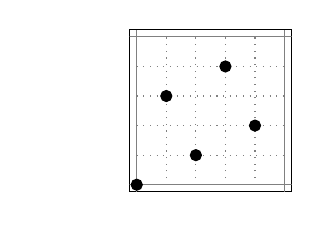
\begin{tikzpicture}
							\begin{axis}[
								plot box ratio = 1 1,
								xmin=-1/21,xmax=22/21,ymin=-1/21,ymax=22/21,
								font=\footnotesize,
								height=0.3\textwidth,
								width=0.3\textwidth,
								xticklabel = \empty,
								yticklabel = \empty,
								ytick style={draw=none},
								xtick style={draw=none},
								]
								\addplot[only marks,black,mark=*,mark size=2pt,mark options={solid}] coordinates {
									(0, 0) (1/5, 3/5) (2/5, 1/5) (3/5, 4/5) (4/5, 2/5)
								};
								\addplot[gray,mark options={solid}] coordinates {
									(0, -0.05) (0, 1.05)
								};
								\addplot[gray,mark options={solid}] coordinates {
									(1.0, -0.05) (1.0, 1.05)
								};
								\addplot[gray,mark options={solid}] coordinates {
									(-0.05, 0) (1.05, 0)
								};
								\addplot[gray,mark options={solid}] coordinates {
									(-0.05, 1.0) (1.05, 1.0)
								};
								\addplot[gray,mark options={solid}, dotted] coordinates {
									(0, 1/5) (1, 1/5)
								};
								\addplot[gray,mark options={solid}, dotted] coordinates {
									(0, 2/5) (1, 2/5)
								};
								\addplot[gray,mark options={solid}, dotted] coordinates {
									(1/5, 0) (1/5, 1)
								};
								\addplot[gray,mark options={solid}, dotted] coordinates {
									(2/5, 0) (2/5, 1)
								};
								\addplot[gray,mark options={solid}, dotted] coordinates {
									(0, 3/5) (1, 3/5)
								};
								\addplot[gray,mark options={solid}, dotted] coordinates {
									(0, 4/5) (1, 4/5)
								};
								\addplot[gray,mark options={solid}, dotted] coordinates {
									(3/5, 0) (3/5, 1)
								};
								\addplot[gray,mark options={solid}, dotted] coordinates {
									(4/5, 0) (4/5, 1)
								};
							\end{axis}
						\end{tikzpicture}
						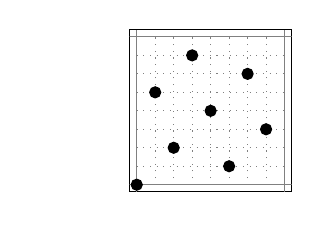
\begin{tikzpicture}
							\begin{axis}[
								plot box ratio = 1 1,
								xmin=-1/21,xmax=22/21,ymin=-1/21,ymax=22/21,
								font=\footnotesize,
								height=0.3\textwidth,
								width=0.3\textwidth,
								xticklabel = \empty,
								yticklabel = \empty,
								ytick style={draw=none},
								xtick style={draw=none},
								]
								\addplot[only marks,black,mark=*,mark size=2pt,mark options={solid}] coordinates {
									(0, 0) (1/8, 5/8) (2/8, 2/8) (3/8, 7/8) (4/8, 4/8) (5/8, 1/8) (6/8, 6/8) (7/8, 3/8)
								};
								\addplot[gray,mark options={solid}] coordinates {
									(0, -0.05) (0, 1.05)
								};
								\addplot[gray,mark options={solid}] coordinates {
									(1.0, -0.05) (1.0, 1.05)
								};
								\addplot[gray,mark options={solid}] coordinates {
									(-0.05, 0) (1.05, 0)
								};
								\addplot[gray,mark options={solid}] coordinates {
									(-0.05, 1.0) (1.05, 1.0)
								};
								\addplot[gray,mark options={solid}, dotted] coordinates {
									(0, 1/8) (1, 1/8)
								};
								\addplot[gray,mark options={solid}, dotted] coordinates {
									(0, 2/8) (1, 2/8)
								};
								\addplot[gray,mark options={solid}, dotted] coordinates {
									(1/8, 0) (1/8, 1)
								};
								\addplot[gray,mark options={solid}, dotted] coordinates {
									(2/8, 0) (2/8, 1)
								};
								\addplot[gray,mark options={solid}, dotted] coordinates {
									(0, 3/8) (1, 3/8)
								};
								\addplot[gray,mark options={solid}, dotted] coordinates {
									(0, 4/8) (1, 4/8)
								};
								\addplot[gray,mark options={solid}, dotted] coordinates {
									(3/8, 0) (3/8, 1)
								};
								\addplot[gray,mark options={solid}, dotted] coordinates {
									(4/8, 0) (4/8, 1)
								};
								\addplot[gray,mark options={solid}, dotted] coordinates {
									(0, 5/8) (1, 5/8)
								};
								\addplot[gray,mark options={solid}, dotted] coordinates {
									(0, 6/8) (1, 6/8)
								};
								\addplot[gray,mark options={solid}, dotted] coordinates {
									(5/8, 0) (5/8, 1)
								};
								\addplot[gray,mark options={solid}, dotted] coordinates {
									(6/8, 0) (6/8, 1)
								};
								\addplot[gray,mark options={solid}, dotted] coordinates {
									(0, 7/8) (1, 7/8)
								};
								\addplot[gray,mark options={solid}, dotted] coordinates {
									(7/8, 0) (7/8, 1)
								};
							\end{axis}
						\end{tikzpicture}
						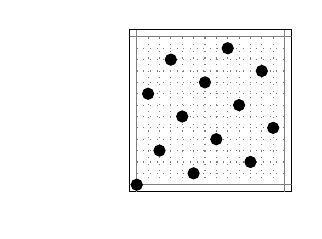
\begin{tikzpicture}
							\begin{axis}[
								plot box ratio = 1 1,
								xmin=-1/21,xmax=22/21,ymin=-1/21,ymax=22/21,
								font=\footnotesize,
								height=0.3\textwidth,
								width=0.3\textwidth,
								xticklabel = \empty,
								yticklabel = \empty,
								ytick style={draw=none},
								xtick style={draw=none},
								]
								\addplot[only marks,black,mark=*,mark size=2pt,mark options={solid}] coordinates {
									(0/13, 0/13) (1/13, 8/13) (2/13, 3/13) (3/13, 11/13) (4/13, 6/13) (5/13, 1/13) (6/13, 9/13) (7/13, 4/13) (8/13, 12/13) (9/13, 7/13) (10/13, 2/13) (11/13, 10/13) (12/13, 5/13)
								};
								\addplot[gray,mark options={solid}] coordinates {
									(0, -0.05) (0, 1.05)
								};
								\addplot[gray,mark options={solid}] coordinates {
									(1.0, -0.05) (1.0, 1.05)
								};
								\addplot[gray,mark options={solid}] coordinates {
									(-0.05, 0) (1.05, 0)
								};
								\addplot[gray,mark options={solid}] coordinates {
									(-0.05, 1.0) (1.05, 1.0)
								};
								\addplot[gray,mark options={solid}, dotted] coordinates {
									(0, 1/13) (1, 1/13)
								};
								\addplot[gray,mark options={solid}, dotted] coordinates {
									(0, 2/13) (1, 2/13)
								};
								\addplot[gray,mark options={solid}, dotted] coordinates {
									(1/13, 0) (1/13, 1)
								};
								\addplot[gray,mark options={solid}, dotted] coordinates {
									(2/13, 0) (2/13, 1)
								};
								\addplot[gray,mark options={solid}, dotted] coordinates {
									(0, 3/13) (1, 3/13)
								};
								\addplot[gray,mark options={solid}, dotted] coordinates {
									(0, 4/13) (1, 4/13)
								};
								\addplot[gray,mark options={solid}, dotted] coordinates {
									(3/13, 0) (3/13, 1)
								};
								\addplot[gray,mark options={solid}, dotted] coordinates {
									(4/13, 0) (4/13, 1)
								};
								\addplot[gray,mark options={solid}, dotted] coordinates {
									(0, 5/13) (1, 5/13)
								};
								\addplot[gray,mark options={solid}, dotted] coordinates {
									(0, 6/13) (1, 6/13)
								};
								\addplot[gray,mark options={solid}, dotted] coordinates {
									(5/13, 0) (5/13, 1)
								};
								\addplot[gray,mark options={solid}, dotted] coordinates {
									(6/13, 0) (6/13, 1)
								};
								\addplot[gray,mark options={solid}, dotted] coordinates {
									(0, 7/13) (1, 7/13)
								};
								\addplot[gray,mark options={solid}, dotted] coordinates {
									(7/13, 0) (7/13, 1)
								};
								\addplot[gray,mark options={solid}, dotted] coordinates {
									(0, 8/13) (1, 8/13)
								};
								\addplot[gray,mark options={solid}, dotted] coordinates {
									(0, 9/13) (1, 9/13)
								};
								\addplot[gray,mark options={solid}, dotted] coordinates {
									(8/13, 0) (8/13, 1)
								};
								\addplot[gray,mark options={solid}, dotted] coordinates {
									(9/13, 0) (9/13, 1)
								};
								\addplot[gray,mark options={solid}, dotted] coordinates {
									(0, 10/13) (1, 10/13)
								};
								\addplot[gray,mark options={solid}, dotted] coordinates {
									(0, 11/13) (1, 11/13)
								};
								\addplot[gray,mark options={solid}, dotted] coordinates {
									(10/13, 0) (10/13, 1)
								};
								\addplot[gray,mark options={solid}, dotted] coordinates {
									(11/13, 0) (11/13, 1)
								};
								\addplot[gray,mark options={solid}, dotted] coordinates {
									(0, 12/13) (1, 12/13)
								};
								\addplot[gray,mark options={solid}, dotted] coordinates {
									(12/13, 0) (12/13, 1)
								};
							\end{axis}
						\end{tikzpicture}
\caption{The $5$-, $8$- and $13$-point Fibonacci lattices.}
\label{fig:fib_lats}
\end{figure}

Of course, Theorem \ref{thm:optimality} is only valuable if we can demonstrate that sufficiently many sets of this form exist. We dedicate the next three subsections to constructing a large number of such sets, starting with the case $d=2$ with particular emphasis on $N=5$, the largest $N$ for which there is such a set in $\mathbb{T}^2$ (see \eqref{eq:div}).  

\subsection{Optimality of the $3$- and $5$-point Fibonacci lattices}

We observe that the 
$5$-point Fibonacci lattice
$$
\Phi_5 = \left\{\left(\frac05, \frac05\right), \left(\frac15, \frac35\right), \left(\frac25, \frac15\right), \left(\frac35, \frac45\right), \left(\frac45, \frac25\right)\right\}
$$
has a single distance vector $\left(\frac15, \frac25 \right)$, see Figure \ref{fig:fib_lats}, in particular $
E_F(\Phi_5) = 20 f\left(\frac15\right) f\left(\frac25\right)
$
as in \eqref{eq:uds_energy}. Therefore, Theorem \ref{thm:optimality} applies in this case and we immediately obtain optimality of this configuration for a variety of potentials.

%\todo[inline]{Label done, but probably could put at another position}

\begin{cor}\label{cor:5}
    If  $\log f$ is $5$-equispacing, then the  $5$-point Fibonacci lattice $\Phi_5$ is an energy minimizer for the corresponding energy $E_F$. In particular, this holds if  (see Proposition \ref{prop:equispaced})
    \begin{itemize}
    \item $f$ is decreasing and logarithmically convex on $(0,1/2]$; or
    \item $f (t) = h (\cos (2\pi t))$ and $\log h$ is absolutely monotone on $[-1,1)$. 
    \end{itemize}
\end{cor}

We further observe that the $5$-point Fibonacci lattice has the lowest energy  among all other $5$-point permutation sets merely under the assumption that $f$ is decreasing  on $(0,1/2]$. 


\begin{lem}\label{lem:5perm}
Assume that $f$ is decreasing  on $(0,1/2]$ (or just that $f(2/5)< f(1/5)$). 
    Then the  $5$-point Fibonacci lattice $\Phi_5$ minimizes the energy $E_F$  among all $5$-point permutation sets.
\end{lem}

\begin{proof}
    We note that permutation sets on $\mathbb{T}^2$ project down to equispaced points on $\mathbb{T}^1$ in both the $x$- and $y$-coordinates. The one-dimensional energy of either of these projections is $5f(1/5)+5f(2/5)$, so the energy of any permutation set in $\mathbb{T}^2$ must be some sum of the form $\sum_{i=1}^{10}a_ib_i$ where five of the $a_i$ are $f(1/5)$, five of the $a_i$ are $f(2/5)$, five of the $b_i$ are $f(1/5)$ and five of the $b_i$ are $f(2/5)$. By the rearrangement inequality \cite{HLP88} we note then that for any permutation set $X$, $$E_F(X)\ge \sum_{i=1}^{10}f(1/5)f(2/5)=10f(1/5)f(2/5),$$ with equality only holding when $f(1/5)=f(2/5)$. Since $10f(1/5)f(2/5)$ is the energy of the $5$-point Fibonacci lattice, we have the desired result. 
\end{proof}


We also notice that the $3$-point Fibonacci lattice  is   equivalent, up to symmetries,  to the diagonal lattice, consisting of points  $\left(0, 0 \right)$, $\left(\frac13, \frac13 \right)$, and   $\left(\frac23, \frac23 \right)$, and has a single distance vector $\left(\frac13, \frac13 \right)$. Thus Theorem \ref{thm:optimality} also applies in this case and yields an identical corollary:

\begin{cor}\label{cor:3}
    If  $\log f$ is $3$-equispacing, then the  $3$-point Fibonacci lattice $\Phi_4$ minimizes the  tensor product  energy $E_F$.
    \end{cor}
   \noindent  A  statement similar to this has already been observed in \cite{Nag25b} and a different proof of this fact in the case when $f$ is logarithmically convex is given in \S\ref{s.type}. 


Finally we would like to mention some other previously known results  about the Fibonacci lattice  and compare them to our results above. All of the prior results concerned specific potentials arising from QMC integration. 

\begin{itemize}
\item It was proved in \cite{Nag25b} that for the potential $f_p$ in \eqref{eq:qmc_potential} with $0 < p \leq 9$ the $5$-point Fibonacci lattice minimizes $E_F(X)$ among all $5$-point configurations. For this particular potential, Corollary \ref{cor:opt_qmc} yields a smaller range of $p \leq 6$. %and even Remark \ref{rem:log_abs_mon} would give the slightly more restrictive $p \leq 8.4992\dots$.
We do however want to point out that the method to prove Theorem \ref{thm:optimality} is completely elementary and does not rely on any computer assisted calculations.

%\todo{Weaker for fib lat but also holds for more point sets!}: It is straight forward to check, as was also already used in \cite{HO16}, that $\log f_p$ is convex for $p \leq 6$. By Proposition \ref{prop:equispaced} (i) we see that $\log f_p$ is $N$-equispacing for this range. However, numerical results suggest that condition (ii) gives a wider range for this potential. To be precise, we conjecture the following:

%For $m, n \in \bbN, n \leq m$ let
%$$
%\kappa(m, n) = 2^{m+1} 3^n \sum_{k=1}^n (-1)^{k-1} (2k-1)! 6^{n-k} {m-k \choose n-k} \cS(m, k)
%$$
%where $\cS(m, k)$ is given by $\sum_{k=1}^m \cS(m,k) x^k = \prod_{j=0}^{m-1} (x+j^2)$. We conjecture that $\kappa(m, n) \in \bbN_0$ for all $1 \leq n \leq m$ and that
%\begin{align*}
%    & \log f_p\left(\frac{\arccos s}{2\pi}\right) \\
%    = & \log\left(1-\frac p{24}\right) + \sum_{m=1}^\infty \frac1{(2m)!} \left(\sum_{n=1}^m \kappa(m, n) p^n (24\pi^2 - (18+\pi^2) p)^{m-n}\right) \left(\frac{s+1}{\pi^2(24-p)}\right)^m
%\end{align*}
%holds uniformly for all $s \in [-1, 1]$. If so, we have that $\log f_p$ is absolutely monotone for $p \leq \frac{24\pi^2}{18+\pi^2} = 8.4992\dots$ and we may apply Proposition \ref{prop:equispaced} (ii) for this range. In particular, we ask if there is a combinatorial interpretation of the numbers $\kappa(m, n)$, i.e. can one construct a combinatorially defined set $M(m, n)$ such that $\kappa(m, n) = \# M(m, n)$. The resemblance of the numbers $\cS(m, k)$ with the (unsigned) Stirling numbers of the first kind \cite[§24.1.3]{AS65} hints at such a connection, also see \cite{GS78}.

%\textcolor{red}{Already discuss this after Theorem 2.3?}

\item Let again $f_p$ be the potential as in \eqref{eq:qmc_potential}. Via an optimization algorithm it was shown in \cite{HO16} that the $N$-point Fibonacci lattice for $N \in \{8, 13\}$ (which has multiple distance vectors, see Figure \ref{fig:fib_lats}) is the energy minimizer for $p \in \{1, 6\}$ among all $N$-point configurations.

%In an earlier paper \cite{HO16} it was shown that if $f(t) = 1 + \frac p2 \left(\frac16 - t + t^2\right)$ with $p \in \{1, 6\}$ and $N \in \{8, 13\}$, then the $N$-point Fibonacci lattice minimizes $E_F(X)$ among all $N$-point configurations.
    \end{itemize}


%\textcolor{red}{It is not clear whether we should actually include all of this here in such detail... Let's discuss} 

\subsection{Classification of lattices with a single distance vector}

In this section we will classify all lattices with a single distance vector. For small values of $N$ this can be checked straightforwardly. Note that for each $N=2, 3, 4$  there is, up to torus symmetry,  %Do we need to define these symmetries?
 only one lattice in $\bbT^d$ with $N$ points:   the corresponding generating vector is 
$$
\left(\frac1N, \dots, \frac1N\right).
$$
The lattices with $N=2, 3$ points are easily seen to %be unique-distance lattices
have a single distance vector, while the case of $N=4$ defines precisely two distance vectors. %In what follows, we may thus only consider lattices with $N \geq 5$ points.

\begin{thm} \label{thm:unique_dist_lat}
    A lattice $\Lambda \sbse [0, 1)^d, \#\Lambda = N \geq 3$ has a single distance vector %is a unique-distance lattice
    if and only if $N$ is prime and the generating vector of $\Lambda$ is of the form (up to torus symmetry)
    $$
    \bigg(\underbrace{\frac1N, \dots, \frac1N}_{m \text{ times}}, \underbrace{\frac2N, \dots, \frac2N}_{m \text{ times}}, \dots, \underbrace{\frac nN, \dots, \frac nN}_{m \text{ times}}\bigg)
    $$
    with $N = 2n+1$ and $d = mn$.
\end{thm}

\begin{proof}
    Let $\Lambda \sbse \bbT^d$ be a %unique-distance 
     lattice with a single distance vector such that $\#\Lambda = N \geq 3$. By applying torus symmetries we may assume the generating vector to have the form
    $$
    \mathbf h = \left(\frac{h_1}N, \dots, \frac{h_d}N\right)
    $$
    with $1 = h_1 \leq \dots \leq h_d \leq \lfloor N/2 \rfloor$. In particular, the distance vector among points in $\Lambda$ must be of the form
    $$
    \dv(\mathbf0, \mathbf h) = \left(\frac{h_1}N, \dots, \frac{h_d}N\right),
    $$
    by Lemma \ref{lem:double_counting} thus
    $$
    \left(\frac{h_1}N, \dots, \frac{h_d}N\right) = \bigg(\underbrace{\frac1N, \dots, \frac1N}_{m \text{ times}}, \underbrace{\frac2N, \dots, \frac2N}_{m \text{ times}}, \dots, \underbrace{\frac nN, \dots, \frac nN}_{m \text{ times}}\bigg)
    $$
    with $n = \frac{N-1}2 \in \bbN$ and $m = \frac{2d}{N-1}$. Furthermore, $N$ must be relatively prime to $1, \dots, \lfloor N/2\rfloor$, so that it must already be prime itself.

    It remains to show that any lattice with generating vector
    $$
    \bigg(\underbrace{\frac1N, \dots, \frac1N}_{m \text{ times}}, \underbrace{\frac2N, \dots, \frac2N}_{m \text{ times}}, \dots, \underbrace{\frac nN, \dots, \frac nN}_{m \text{ times}}\bigg)
    $$
    with $d=mn$ and $N=2n+1$ prime is a lattice with a single distance vector. Indeed, for an arbitrary $k \in \{1, \dots, N-1\}$ consider the distance vector from $\mathbf{0} = (0, \dots, 0)$ to
    $$
    \bx^k = \left(\left\{\frac{h_1 k}N\right\}, \dots, \left\{\frac{h_d k}N\right\}\right)
    $$
    with $h_1 = \dots = h_m = 1, h_{m+1} = \dots = h_{2m} = 2, \dots, h_{(n-1)m+1} = \dots = h_{nm} = n$. We will show that this distance vector does not depend on $k$. If there were $h, \tilde h \in \{1, \dots, n\}, h \neq \tilde h$ with
    $$
    \left\{\frac{hk}N\right\} = \left\{\frac{\tilde hk}N\right\},
    $$
    then we would either get
    $$
    hk \equiv \tilde h k \mod N \quad \Rightarrow \quad h = \tilde h
    $$
    or
    $$
    hk \equiv N - \tilde h k \mod N \quad \Rightarrow \quad (h + \tilde h) k \equiv 0 \mod N \quad \Rightarrow \quad h + \tilde h = N,
    $$
    both leading to contradictions since $h \neq \tilde h$ and $h + \tilde h \leq 2n < N$. Thus
    $$
    \dv(\mathbf 0, \bx^k) = \bigg(\underbrace{\frac1N, \dots, \frac1N}_{m \text{ times}}, \underbrace{\frac2N, \dots, \frac2N}_{m \text{ times}}, \dots, \underbrace{\frac nN, \dots, \frac nN}_{m \text{ times}}\bigg)
    $$
    and by the lattice structure this is also the distance vector between any other two point from the lattice.
\end{proof}

We see that if $2d+1$ is prime, the bound on $N$ mentioned after \eqref{eq:div} can be attained by such a lattice construction.

%\textcolor{red}{More generally: the number of distance vectors, that the lattice given by the generating vector $(k: 1 \leq k \leq N/2, \gcd(k, N) = 1)$ defines, is the number of proper factors of $N$.}

\subsection{Some non-lattice  sets with a single distance vector}

In addition to the lattices from the previous section, we can also construct  the following $4$-, $6$-, $8$-, and $9$-point Latin hypercube sets with a single distance vector in $\bbT^3$, $\bbT^{10}$, $\bbT^{14}$, and $\bbT^{12}$ respectively:
\begin{align*}
    X_4 = \left\{\frac14 (0, 0, 0), \frac14 (1, 1, 2), \frac14 (2, 3, 1), \frac14 (3, 2, 3)\right\},
\end{align*}

\begin{align*}
    X_6 = \bigg\{ & \frac16 (0, 0, 0, 0, 0, 0, 0, 0, 0, 0), \frac16 (1, 1, 1, 1, 2, 2, 2, 2, 3, 3), \\
    & \frac16 (2, 2, 2, 3, 3, 4, 5, 5, 1, 1), \frac16 (3, 3, 4, 2, 5, 1, 1, 4, 4, 5), \\
    & \frac16 (4, 5, 3, 4, 1, 3, 4, 1, 5, 4), \frac16 (5, 4, 5, 5, 4, 5, 3, 3, 2, 2) \bigg\},
\end{align*}

\begin{align*}
    X_8 = \bigg\{ & \frac18 (0, 0, 0, 0, 0, 0, 0, 0, 0, 0, 0, 0, 0, 0), \frac18 (1, 1, 1, 1, 2, 2, 2, 2, 3, 3, 3, 3, 4, 4), \\
& \frac18 (2, 2, 3, 5, 1, 4, 4, 5, 1, 6, 6, 7, 1, 3), \frac18 (3, 3, 2, 4, 3, 6, 6, 7, 6, 1, 1, 4, 5, 7), \\
& \frac18 (4, 5, 6, 3, 5, 1, 5, 1, 2, 4, 7, 1, 2, 6), \frac18 (5, 4, 7, 2, 7, 3, 7, 3, 5, 7, 4, 6, 6, 2), \\
& \frac18 (6, 7, 5, 6, 4, 5, 1, 4, 7, 2, 5, 2, 3, 1), \frac18 (7, 6, 4, 7, 6, 7, 3, 6, 4, 5, 2, 5, 7, 5)\bigg\},
\end{align*}

\begin{align*}
    X_9 = \bigg\{ & \frac19 (0, 0, 0, 0, 0, 0, 0, 0, 0, 0, 0, 0), \frac19 (1, 1, 1, 2, 2, 2, 3, 3, 3, 4, 4, 4), \\
& \frac19 (2, 2, 2, 4, 4, 4, 6, 6, 6, 8, 8, 8), \frac19 (3, 4, 5, 1, 6, 8, 1, 4, 7, 2, 3, 7), \\
& \frac19 (4, 3, 8, 7, 8, 6, 2, 8, 5, 5, 7, 3), \frac19 (5, 6, 4, 8, 1, 3, 4, 7, 1, 7, 2, 6), \\
& \frac19 (6, 5, 7, 5, 3, 1, 5, 2, 8, 1, 6, 2), \frac19 (7, 8, 3, 6, 5, 7, 7, 1, 4, 3, 1, 5), \\
& \frac19 (8, 7, 6, 3, 7, 5, 8, 5, 2, 6, 5, 1)\bigg\}.
\end{align*}
These point sets are again energy minimizers in the sense of Theorem \ref{thm:optimality}. It can be observed that $X_4$ and $X_8$ are digital nets \cite{DP10}.

It is easy to see that for every $N \in \bbN$ there exists a Latin hypercube set  $X \sbse \bbT^d, \#X = N$ with a single distance vector in dimension $d = (N-1)!$, namely where every coordinate of $\bbT^{(N-1)!}$ corresponds to a permutation $\sigma$ of $\{0, 1,\dots, N-1\}$ fixing $\sigma(0) = 0$. It is thus more interesting to find, for any given $N \in \bbN$, the smallest dimension $d = d(N)$ for which there exists an $N$-point Latin hypercube set with a single distance vector in $\bbT^d$. The condition \eqref{eq:div} is necessary but not sufficient.

\section{Energy minimizers have distinct coordinates}\label{s.noequal}

In the present section we  demonstrate that, under very mild assumptions on the function $f$, both global and local energy minimizers must necessarily have distinct coordinates. For example, in the two-dimensional case $\bbT^2$ this implies no two points in  the minimizing configuration can lie on the same horizontal or vertical line. This brings us one step closer to understanding when permutation sets or Latin hypercube sets minimizer tensor product energies. The result is formalized in the following theorem:


\begin{thm}\label{prop:coordinate_improvement}
	Let $f: \mathbb R  \rightarrow (0, \infty)$ be continuous, $1$-periodic, even and satisfy the following assumptions:
	\begin{itemize}		
		\item [(i)] $f(t)$ is differentiable on $(0, 1)$, %and ...
		
		\item [(ii)] there are constants $C > 0$ and  $\varepsilon > 0$ such that  $f(t) \leq f(0) - Ct$ for all $0 \leq t < \varepsilon$. %(that is the function $x \mapsto f(|x|)$ fulfils the assumptions of $F$ as in Lemma \ref{lem:basic_calculcus_lemma}).
	\end{itemize}
	Consider an $N$-point configuration  $X = \{\bx^0, \dots, \bx^{N-1}\} \subseteq \bbT^d$ such that $x^0_1 = \dots = x^j_1$ for some  $j \geq 1$ and $x^k_1 \neq x^0_1$ for all $k > j$ (if such $k$ exist). %Then there is a number  $-1 \leq t \leq 1$ such that for
	Define a perturbation of $X$ by
    $$
	X_r \coloneqq \{\bx^0(r), \bx^1, \dots, \bx^{N-1}\},
	$$
    where $\bx^0(r) = (x_1^0 + r, x_2^0, \dots, x_d^0)$ for $r \in [-1/2, 1/2)$. Then the function
    $$
    r \mapsto E_F(X_{r})
    $$
    does not have a local minimium at $r=0$.
	\end{thm}

As a direct consequence we obtain the following.

\begin{cor}\label{c.noequal}
    Let $f$ satisfy the assumptions of Theorem \ref{prop:coordinate_improvement} and let $X = \{\bx^0, \bx^1, \dots, \bx^{N-1}\} \sbse \bbT^d$ be a (local) minimizer of the corresponding energy $E_F$. Then
    $$
    x_i^k \neq x_i^\ell
    $$
    for all $i = 1, \dots, d$ and $k, \ell = 0, 1, \dots, N-1, k \neq \ell$.
\end{cor}

%I think we might want the corollary as the theorem here, and the result in the theorem is just the method used to prove the corollary. As it's written, the theorem is a little hard to read.

That is, points in minimizing configurations must necessarily have distinct coordinates.

\begin{rem*}
Assumption (ii) in Theorem  \ref{prop:coordinate_improvement} (which means that $f$ has a sharp kink at $t=0$) can be interpreted as saying that the repulsion induced by the interaction $F$ is quite strong at small distances in each coordinate. 
We observe that if $f$ is singular at zero, i.e. $f(0) = + \infty$, the statement of Corollary \ref{c.noequal}  would have been obvious. It is a known phenomenon \cite{CFP} that when the local repulsion is weak, then minimizers of energies tend to cluster. Thus, this result can be viewed as complimentary: minimizers do not cluster when the local repulsion is strong. %We intend to further explore this phenomenon in subsequent work. 

Observe that assumption (ii) is satisfied by various natural kernels, in particular the aforementioned $f(t) = 1/2 - t + t^2$ for $t\in [0,1]$ which corresponds to the periodic $L_2$-discrepancy, or more generally the QMC potential \eqref{eq:qmc_potential} for $0 < p < 24$ (where it stays positive). 
\end{rem*}


To prove Theorem  \ref{prop:coordinate_improvement}, we begin with a simple   observation: if a function has a downwards-opening kink, then it  cannot have a local minimum there.


\begin{lem} \label{lem:basic_calculcus_lemma}
	Let $G: (-\varepsilon, \varepsilon) \rightarrow \mathbb{R}$ be a function with $G(r) \leq G(0) - C|r|$ in $-\varepsilon < r < \varepsilon$ for some $C > 0$. Let $H: (-\varepsilon, \varepsilon) \rightarrow \mathbb{R}$ be   differentiable at $r = 0$. Then $r \mapsto G(r) + H(r)$ does not have a local minimum at $r = 0$.
\end{lem}


%A particular example of such a potential would be given by the potential of the periodic $L_2$-discrepancy.

\begin{proof} [Proof of Theorem \ref{prop:coordinate_improvement}]
    Without loss of generality let  $x^0_1 = \dots = x^j_1=0$ be the common coordinate. Consider the perturbation $\bx^0(r) = (r, x_2^0, \dots, x_d^0)$ while keeping all other coordinates fixed. We separate the terms of $E_F (X_r)$ that depend on $r$ and treat the rest as a constant $K_1>0$
	\begin{align*}
		E_F (X_r ) = & f(r) \cdot 2\sum_{k = 1}^{j} \prod_{i=2}^d f(x_i^0-x_i^k) 
		 +  2\sum_{k = j+1}^{N-1} f(r - x_1^k) \prod_{i=2}^d f(x_i^0-x_i^k) + K_1.
	\end{align*}
	Let
	$$
	G(r) = f(r) \cdot 2\sum_{k = 1}^{j} \prod_{i=2}^d f(x_i^0-x_i^k)
    $$
    and
    $$
	H(r)  =  2\sum_{k = j+1}^{N-1} f(r - x_1^k) \prod_{i=2}^d f(x_i^0-x_i^k) + K_1.
	$$
	By (i) and since $x_1^k \neq 0$ for $k > j$ we have that $H(r)$ is differentiable at $r=0$. Also note that
	$$
    K_2 = 2\sum_{k = 1}^{j} \prod_{i=2}^d f(x_i^0-x_i^k) > 0
	$$
	is a positive constant since $f$ only takes on positive values and $j \geq 1$ so that the sum is nonempty. Hence (ii) implies that
	$$
	G(r) \leq K_2 (f(0) - C |r|)  = G(0) - C K_2 |r|
	$$
	in a neighborhood around $r = 0$. Thus $G$ and $H$ satisfy the assumptions of Lemma \ref{lem:basic_calculcus_lemma}, hence $E_F (X_r) = G(r) +H(r)$ does not have a local minimum in $r=0$.
\end{proof}


%\begin{rem*}
%	It would be of significant interest if one can get a quantitative result on the separation of the points of (local or global) minimizers. In general, one cannot hope for global minimizers to be perfectly equispaced, i.e. Latin hypercube sets, see []. However, it seems imaginable that under certain assumptions on the potential function $f$ (such as logarithmic convexity or other decay conditions) one could be able to control the difference of the coordinates of consecutive points in a meaningful way.
%\end{rem*}

%\todo[inline]{I AM NOT SURE ABOUT THE LAST REMARK ABOVE. Can probably replace the differentiability assumptions by bounds on the left- and right-derivative, so that we do not need the differentiability assumption for convex $f$. Although this would be a distinct case from the one discussed above and would need a slightly different proof.}
    %We could leave this as a remark but the writing would need to be formalized.


\section{Permutation type and winding number}\label{s.type}

In this section  we show that lattices minimize tensor product energies with logarithmically convex potential $f$  among large classes of sets which share structural similarities with the lattice. In particular, lattices are local minimizers of such energies. To this end, we prove a lower bound on the energy in terms of the permutation type of the configuration. 


Given a point set in  $\mathbb T^d \simeq[0,1)^d$, we can always assume that the $x_1$-coordinates are ordered, i.e. $x_1^k\le x_1^\ell$ for $k<\ell$. However the same need not hold for the other coordinates. Instead when $d\ge 2$ we can order the points by one of the other coordinates and obtain a permutation that relates this ordering to our original ordering. We obtain the following definition:
\begin{defi}\label{def.perm_type}
    For a given point set $X = \{ \bx^0, \bx^1, \dots, \bx^{N-1} \} \subset \mathbb T^d \simeq[0,1)^d$, suppose $S=(\sigma_1,\sigma_2,\dots,\sigma_d)$ is a $d$-tuple of permutations of $\{0,1,\dots,N-1\}$ satisfying
    $$
    x_i^{\sigma^{-1}_i(0)}\le x_i^{\sigma^{-1}_i(1)}\le\dots\le x_i^{\sigma^{-1}_i(N-1)}
    $$
    for all $i$. Then we say $S$ is a \emph{permutation type} of $X$.
\end{defi}

For example, we note that the Latin hypercube set $X_{\sigma_2,...,\sigma_d}$ given in Definition \ref{def:lat_hypcube} has permutation type $(\text{id},\sigma_2,...,\sigma_d)$. We will generally assume that the first coordinates are ordered, i.e. $\sigma_1$ is the identity permutation, and by translating so that $\bx^0=(0,0,...,0)$ we will also assume that $\sigma_i(0)=0$ for all $i$. The permutation type is uniquely defined if and only if all points have distinct coordinates in the sense of §\ref{s.noequal}. For any permutation $\sigma$ we will define the \emph{$k$-th winding number} associated with $\sigma$ by $$\omega_\sigma(k):=\#\{j:\sigma((j+k) \textup{ mod } N)<\sigma(j)\}.$$ %We will define $\omega_\sigma(0)=0$\todo{do we need that?}.
For notational simplicity,  input values outside of the domain of $\sigma$ will be implicitly assumed to be taken modulo $N$. Conceptually, this quantity counts how many times the permutation winds around the torus, moving along it with step size $k$. With this definition we are now ready to state the lower bound for the energy.

\begin{thm}\label{thm:permtype}
    Assume the configuration  $X=\{ \bx^0, \bx^1,\dots,\bx^{N-1} \} \subset \mathbb T^d $ has unique permutation type $(\sigma_1,\sigma_2,\dots,\sigma_d)$. Then the following inequality holds for all  potentials $f$ decreasing and logarithmically convex on $(0,1/2]$:
    $$E_F(\bx^0,\dots,\bx^{N-1})\ge N\sum_{k=1}^{N-1}\prod_{i=1}^df\left(\frac{\omega_{\sigma_i}(k)}{N}\right).$$
    If $f$ is strictly decreasing, equality is obtained if and only if the point set $X = \{ \bx^0, \bx^1,\dots,\bx^{N-1} \}$ is a lattice.
\end{thm}



\begin{proof}
    By regrouping the terms,  the energy can be written in the form \begin{equation}\label{eq:perm_energy}
        E_F(\bx^0,\dots,\bx^{N-1})=\sum_{\ell=1}^{N-1}\sum_{k=0}^{N-1} F(\bx^k-\bx^{k+\ell}),
    \end{equation}
    if we identify $\bx^{k+\ell}=\bx^{k+\ell-N}$ in the case $k+\ell>N-1$. For $x,y \in [0,1) \simeq \mathbb T$ we define
    $$
    \delta_\circlearrowleft(x,y)=\begin{cases}
        y-x, & y \geq x, \\
        1+y-x, & y < x,
    \end{cases}
    $$
    which can be thought of as the \emph{counterclockwise} geodesic distance. Note that this need not always equal the geodesic distance $\delta$ defined in \eqref{eq:geod_dist}, but the periodicity and evenness of $f$ implies  that the value of  $f$ is independent of the choice between these two distances as its argument. Thus we rewrite 
    \begin{equation*}
    F\left(\bx^k-\bx^{k+\ell}\right)=\prod_{i=1}^df\left(x_i^k-x_i^{k+\ell}\right)  = \prod_{i=1}^df\left(\delta_\circlearrowleft(x_i^k,x_i^{k+\ell})\right).\end{equation*}
    Since $f$ is logarithmically convex and decreasing on $(0,1/2]$, it is log-convex on $(0,1)$, and hence  
    the function $F$ is convex as a function of $d$ variables on $(0,1)^d$. Therefore, we can apply  Jensen's inequality to the inner sum in  the right-hand side of \eqref{eq:perm_energy} and we obtain %the following inequality:
     \begin{align}\label{eq:jensens}
     \begin{split}
         E_F(\bx^0,\dots,\bx^{N-1}) &  =  \sum_{\ell=1}^{N-1} \sum_{k=0}^{N-1} F \left( \delta_\circlearrowleft(x_1^k,x_1^{k+\ell}), \dots, \delta_\circlearrowleft(x_d^k,x_d^{k+\ell} )\right)\\ & \ge N\sum_{\ell=1}^{N-1}F\left(\frac{1}{N}\sum_{k=0}^{N-1}\delta_\circlearrowleft(x_1^k,x_1^{k+\ell}),\dots,\frac{1}{N}\sum_{k=0}^{N-1}\delta_\circlearrowleft(x_d^k,x_d^{k+\ell})\right)\\
    & = N\sum_{\ell=1}^{N-1}\prod_{i=1}^d f\left(\frac{1}{N}\sum_{k=0}^{N-1}\delta_\circlearrowleft(x_i^k,x_i^{k+\ell})\right).
     \end{split}
    \end{align}
    %We recall that $f$ is $1$-periodic so for two values $x,y\in[0,1)$ we define
   % and rewrite $F(\bx_i-%\bx_{i+j})=f(x_i-x_{i+j})f(y_i-y_{i+j})$ as $f(d(x_i,x_j))f(d(y_i,y_j))$. Then since $F$ is convex, by using Jensen's inequality on the right-hand side of \ref{eq:perm_energy} we obtain the following inequality: \begin{equation}\label{eq:jensens}E_F(\bx_0,...,\bx_{N-1})\ge N\sum_{i=0}^{N-1}F\left(\frac{1}{N}\sum_{j=0}^{N-1}(d(x_j,x_{i+j}),d(y_j,y_{i+j}))\right).\end{equation}
 Observe that $\delta_\circlearrowleft(x_i^k,x_i^{k+\ell})= 1+x_i^{k+\ell}-x_i^k$ if and only if 
 %$x_{i+j}<x_j\Rightarrow i+j\ge N$ 
 $x_i^{k+\ell}<x_i^k$, i.e.  $x_i^{\sigma^{-1}_i(\sigma_i(k+\ell))}<x_i^{\sigma^{-1}_i(\sigma_i(k))}$, which is equivalent to  $\sigma_i(k+\ell)<\sigma_i(k)$. This  occurs for $\omega_{\sigma_i}(\ell)$ values of $k$ (note that unique permutation type means that we can ignore the case of equality between coordinates). Otherwise it equals $x_i^{k+\ell}-x_i^k$. Telescoping the sum, we  conclude that 
 $$ \sum_{\ell=0}^{N-1}\delta_\circlearrowleft(x_i^k,x_i^{k+\ell}) = {\omega_{\sigma_i}(k)},$$ and thus, as desired,  $$E_F(\bx^0,\dots,\bx^{N-1})\ge N\sum_{k=1}^{N-1}\prod_{i=1}^df\left(\frac{\omega_{\sigma_i}(k)}{N}\right).$$
    
    Finally, we note that there are two cases for equality in Jensen's inequality in \eqref{eq:jensens}: either $f$ is linear on the relevant domain (which cannot be the case if $f$ is strictly decreasing and logarithmically convex on $(0,1/2]$) or the argument of $F$ is independent of $k$, i.e. \begin{equation*}%\label{eq:jensens_condition}
       \delta_\circlearrowleft(x_i^k-x_i^{k+\ell})=\delta_\circlearrowleft(x_i^{k'}-x_i^{k'+\ell})\text{ for all }i, \ell, k,k' ,
    \end{equation*} which by their periodic structure is fulfilled by lattices. Conversely, if this condition is satisfied we note that since a unique permutation type means none of the coordinates coincide, the $\ell=1$ case implies that our configuration is a lattice. This proves the desired equivalence.%\todo[inline]{DB: Should we elaborate on this? The statement that ``$\bx^j-\bx^{i+j}$ is the same vector for all $j$'' only holds up to changes of signs in each coordinate, so it could be a little more delicate.
    %NN: But then we wouldn't have a permutation set, as a coordinate would be repeated, so this case does not occur.}
  %  The right-hand side of \ref{eq:jensens} is equivalent to $$N\sum_{i=0}^{N-1}f\left(\frac{1}{N}\sum_{j=0}^{N-1}d(x_j,x_{i+j})\right)f\left(\frac{1}{N}\sum_{j=0}^{N-1}d(y_j,y_{i+j})\right).$$
\end{proof}

We immediately obtain the following corollary:

\begin{cor}\label{cor:lat_type}
Assume that the potential $f$ is decreasing and logarithmically convex on $(0,1/2]$. Let $X \subset \mathbb T^d$ be an $N$-point integration lattice, and let $Y \subset \mathbb T^d$ be an $N$-point configuration with the same permutation type as $X$. Then $$ E_F (Y) \ge E_F (X).$$
\end{cor}

In other words, lattices minimize the energy among all sets with the same permutation type. Observing that a  small perturbation of a lattice does not change the  permutation type, we arrive directly at local optimality. %We note that it might be possible, but very technical in general, to obtain this result using the standard variational methods.

\begin{cor}\label{cor:lattice}
   If a point set $X$ is a lattice and $f$ is decreasing and logarithmically convex on $(0,1/2]$, then $X$ is a local minimum of $E_F$.
\end{cor}



The last two corollaries  exhibit an example of the behavior discussed in the introduction: certain permutation sets (namely, lattices) minimize the energy among large classes of more general (non-permutation) sets. 

Finally we note that the case  $N=3$ can also be addressed by these methods because this case has only two permutation types in each coordinate, and all permutation sets in this case are lattices (up to the symmetries of the torus). Thus a special case of  Corollary \ref{cor:3} when $f$ is logarithmically convex, can be obtained as a consequence of Corollary \ref{cor:lat_type}. %Theorem \ref{thm:permtype} (or rather Corollary \ref{cor:lat_type}).

%\begin{cor}\label{c.N3}
%    For $N=3$, when $f$ is log-convex any permutation set minimizes $E_F$.
%\end{cor}



\section{The cases $N=4$ and $N=6$ in $\mathbb{T}^2$}\label{sec:N4}

In the setting of $\mathbb{T}^2$, the cases $N=4$ and $N=6$ are unique: the only possible lattices are the identity lattice that places all points on $y=x$, and its reflection that places all points on $y=1-x$. However, unlike in the case $N=3$ (which like $N=5$ is covered by Corollary \ref{cor:3}) there are other permutation sets that are not one of these two cases. %In general, we have the following result for the energy of the identity permutation set.

We first observe that the permutation set whose permutation type is the identity cannot strictly minimize the  energy, even among permutation sets. 

%, and by a simple rearrangement inequality we can see that if $f$ is decreasing on $(0,1/2]$ then these two lattices must have a higher energy than any other possible permutation set.

\begin{prop} \label{prop:id}
    Let $N \in \bbN$ and let $f: \bbT \rightarrow [0, \infty)$ be a potential. 
    Then, for all permutations $\sigma$ of $\{0, 1, \dots, N-1\}$,
     we have
    $$
    E_F(X_{\id}) \geq E_F(X_\sigma),
    $$
    where $\id$ denotes the identity permutation and $X_\sigma$ is a permutation set with permutation type $\sigma$
     (see \eqref{e.permutation}).
\end{prop}

%\todo[inline]{N: If I'm not mistaken we actually do not need decreasing in $(0, 1/2]$, do we?}

\begin{proof}
    The energy of $X_\sigma$ takes the form
    $$
    E_F(X_\sigma) = \sum_{\substack{k, \ell = 0 \\ k \neq \ell}}^{N-1} f\left(\frac{k-\ell}N\right) f\left(\frac{\sigma(k)-\sigma(\ell)}N\right).
    $$
    As multisets we have
    \begin{align*}
        & \left\{f\left(\frac{k-\ell}N\right): k, \ell \in \{0, 1, \dots, N-1\}, k \neq \ell\right\} \\
        = & \left\{f\left(\frac{\sigma(k)-\sigma(\ell)}N\right): k, \ell \in \{0, 1, \dots, N-1\}, k \neq \ell\right\},
    \end{align*}
    by the rearrangement inequality \cite{HLP88} the energy $E_F$ is thus maximized if
    $$
    f\left(\frac{k-\ell}N\right) = f\left(\frac{\sigma(k)-\sigma(\ell)}N\right)
    $$
    for all $k, \ell$, which is the case for the identity permutation.
\end{proof}

Thus, for $N=4$ and $6$, candidates for energy minimizers must be something other than a lattice. We shall consider these cases in detail. %However in these settings the point configurations considered still have a very small distance vector set, recalling the sharp configurations of \cite{CK07}. 

\subsection{The $N=4$ case}

In the case $N=4$, up to symmetries of the torus, there is only one other permutation set besides the identity permutation, namely
\begin{align} \label{opt_4_perm}
    X^{(4)} \coloneqq \{(0,0),(1/4,1/2),(1/2,1/4),(3/4,3/4)\},
\end{align}
which by Proposition \ref{prop:id} minimizes the energy among all $4$-point permutation sets. If $f$ is differentiable on $(0, 1)$, %then $E_F$ is smooth as a function of the point configuration (when coordinates of the points do not coincide), and we are able to 
one can perform gradient descent to approach a local minimizer. Following off of an observation in \cite{HO16} we claim that with appropriate convexity conditions this will actually yield a global minimizer, and we present a simple condition how to determine it.

\begin{prop}\label{prop:n4}
    Let  $f$ be differentiable on $(0,1)$, as well as decreasing   and logarithmically convex on $(0,1/2]$. Then there exists an $a\in(0,1/2)$ such that the $4$-point configuration $$X_a^{(4)}\coloneqq\{(0,0),(a,1/2),(1/2,a),(1/2+a,1/2+a)\}$$  is a  minimizer of $E_F$. This value of $a$ satisfies \begin{equation}\label{eq:n4_condition}
        f'(a)f(1/2)=f'(1/2-a)f(1/2-a).
    \end{equation}
    If $f$ is strictly logarithmically convex, this value of $a$ is unique.
\end{prop}

We would like to point out that in \cite{HO16}  such a set was obtained as the energy minimizer of $E_F$ with  $f(t) = \frac12 - t + t^2$ (Fig. \ref{fig:four_configs}) using a proof assisted with numerics. Proposition \ref{prop:n4} provides a simple way to find such minimizers for a wide range of potentials and admits a transparent proof, which we now present. 


\begin{proof}
    We note that $f$ being logarithmically convex results in the tensor product potential $F$ being convex on $(0,1)\times(0,1)$, see \cite{SS12b}. This means that as a function of $\bx^i$ and $\bx^j$, the expression $F(\bx^i-\bx^j)$ is convex when the order  of the $x$- and $y$-coordinates of the two points is fixed. Since the sum of convex functions is convex, we  conclude that $E_F$ is convex as a function of the coordinates of our three unfixed points (we assume $\bx^0=(0,0)$) when we restrict it to point configurations of a specific permutation type. Viewing the coordinates of our three unfixed points as an element of $[0,1)^6$, we observe that a convex combination of two element in this space that are of the same permutation type will result in another element of the same permutation type. Therefore the set of all configurations of the same permutation type is a convex set and thus any local minimizer of $E_F$ in this set is a minimizer among all point sets of the same permutation type.

\begin{figure}[htp]
\hspace{1.1cm}
						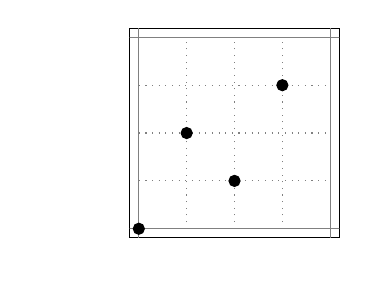
\begin{tikzpicture}
							\begin{axis}[
								plot box ratio = 1 1,
								xmin=-1/21,xmax=22/21,ymin=-1/21,ymax=22/21,
								font=\footnotesize,
								height=0.35\textwidth,
								width=0.35\textwidth,
								xticklabel = \empty,
								yticklabel = \empty,
								ytick style={draw=none},
								xtick style={draw=none},
								]
								\addplot[only marks,black,mark=*,mark size=2pt,mark options={solid}] coordinates {
									(0, 0) (1/4, 1/2) (1/2, 1/4) (3/4, 3/4)
								};
								\addplot[gray,mark options={solid}] coordinates {
									(0, -0.05) (0, 1.05)
								};
								\addplot[gray,mark options={solid}] coordinates {
									(1.0, -0.05) (1.0, 1.05)
								};
								\addplot[gray,mark options={solid}] coordinates {
									(-0.05, 0) (1.05, 0)
								};
								\addplot[gray,mark options={solid}] coordinates {
									(-0.05, 1.0) (1.05, 1.0)
								};
								\addplot[gray,mark options={solid}, dotted] coordinates {
									(0, 1/4) (1, 1/4)
								};
								\addplot[gray,mark options={solid}, dotted] coordinates {
									(0, 1/2) (1, 1/2)
								};
								\addplot[gray,mark options={solid}, dotted] coordinates {
									(1/4, 0) (1/4, 1)
								};
								\addplot[gray,mark options={solid}, dotted] coordinates {
									(1/2, 0) (1/2, 1)
								};
								\addplot[gray,mark options={solid}, dotted] coordinates {
									(0, 3/4) (1, 3/4)
								};
								\addplot[gray,mark options={solid}, dotted] coordinates {
									(3/4, 0) (3/4, 1)
								};
							\end{axis}
						\end{tikzpicture}
						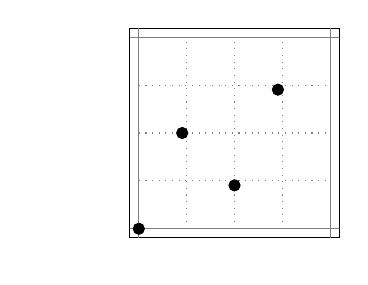
\begin{tikzpicture}
							\begin{axis}[
								plot box ratio = 1 1,
								xmin=-1/21,xmax=22/21,ymin=-1/21,ymax=22/21,
								font=\footnotesize,
								height=0.35\textwidth,
								width=0.35\textwidth,
								xticklabel = \empty,
								yticklabel = \empty,
								ytick style={draw=none},
								xtick style={draw=none},
								]
								\addplot[only marks,black,mark=*,mark size=2pt,mark options={solid}] coordinates {
									(0, 0) (0.226698825758202, 1/2) (1/2, 0.226698825758202) (0.726698825758202, 0.726698825758202)
								};
								\addplot[gray,mark options={solid}] coordinates {
									(0, -0.05) (0, 1.05)
								};
								\addplot[gray,mark options={solid}] coordinates {
									(1.0, -0.05) (1.0, 1.05)
								};
								\addplot[gray,mark options={solid}] coordinates {
									(-0.05, 0) (1.05, 0)
								};
								\addplot[gray,mark options={solid}] coordinates {
									(-0.05, 1.0) (1.05, 1.0)
								};
								\addplot[gray,mark options={solid}, dotted] coordinates {
									(0, 1/4) (1, 1/4)
								};
								\addplot[gray,mark options={solid}, dotted] coordinates {
									(0, 1/2) (1, 1/2)
								};
								\addplot[gray,mark options={solid}, dotted] coordinates {
									(1/4, 0) (1/4, 1)
								};
								\addplot[gray,mark options={solid}, dotted] coordinates {
									(1/2, 0) (1/2, 1)
								};
								\addplot[gray,mark options={solid}, dotted] coordinates {
									(0, 3/4) (1, 3/4)
								};
								\addplot[gray,mark options={solid}, dotted] coordinates {
									(3/4, 0) (3/4, 1)
								};
							\end{axis}
						\end{tikzpicture}
\caption{The best $4$-point permutation set and the energy minimizer $X_a^{(4)}$ for the potential $f(t) = \frac12 - t + t^2$. Here, $a = 0.22669\dots$ is the solution to the cubic equation $2a^3+a-\frac14=0$.}
\label{fig:four_configs}
\end{figure}

    From Corollary \ref{cor:lat_type} we know that the identity lattice minimizes the energy among sets of the same permutation type, however by Proposition \ref{prop:id} it will not be a (unique) minimizer among all $4$-point configurations in $\bbT^2$. Considering torus symmetries, we need to check only one other permutation type, namely the one of $X_a^{(4)}$. Thus, we only need to show that, for $a$ satisfying \eqref{eq:n4_condition}, $X_a^{(4)}$ is stationary with respect to $E_F$ in order to demonstrate  that it is an energy minimizer. For this, we consider the gradient of the energy functional $E_F(\mathbf 0, \bx^1, \bx^2, \bx^3)$ in terms of the $6$ variables $\bx^1 = (x_1^1, x_2^1)$, $\bx^2=(x_1^2, x_2^2)$, $\bx^3=(x_1^3, x_2^3)$. Taking the partial derivative with respect to any of these $6$ coordinates, we see that it is $0$ if and only if \eqref{eq:n4_condition} holds. We thus conclude that $X_a^{(4)}$ is a minimizer. We know such an $a$ exists because $$E_F(X_a^{(4)})=4f(a)f(1/2)+2f(1/2-a)^2$$ is a convex function in $a$ and thus must have a minimum (the cases of $a=0$ and $a=1/2$ are not minimizers by Corollary \ref{c.noequal}). If $f$ is strictly logarithmically convex then $E_F(X_a^{(4)})$ is a strictly convex function of $a$ and has a unique minimizer, so \eqref{eq:n4_condition} is satisfied by only one value of $a$.
\end{proof}

With this result we reduce the complexity of the problem down to a single variable, making it much more approachable for potentials satisfying the given condition. If we consider the potential given in \eqref{eq:qmc_potential}, for example, we find that the energy minimizer is $X_a^{(4)}$ with $a = a(p)$ satisfying the cubic
$$
\frac{p^2}2a^3+2p\left(1-\frac p{24}\right)a-\frac p2\left(1-\frac p{24}\right) = 0.
$$
It can be noted that for $0 < p \leq 6$, where \eqref{eq:qmc_potential} is logarithmically convex, we have $|a(p)-\frac14| < 0.024$. This phenomenon, that global optimizers do not stray too far from permutation sets, was first observed in \cite{HO16}. Figure \ref{fig:four_configs} shows the global minimizer for the concrete potential of the periodic $L_2$-discrepancy, equivalently $p=6$ above.

\begin{rem}\label{rem:n4not}
We finish this subsection by noting that the permutation set \eqref{opt_4_perm}, i.e. $X_{1/4}^{(4)}$, will only satisfy the condition given in \eqref{eq:n4_condition} if $f(1/2)=f(1/4)$, in which case it will also yield the same energy as the identity permutation. Thus, for potentials that satisfy the conditions of Proposition \ref{prop:n4}, there cannot be a unique energy minimizer that is a permutation set.
\end{rem}

%\begin{prop}
%If $f$ is differentiable on $(0,1)$ and $f(1/2)<f(1/4)$, then the above $X$ is not a local energy minimizer.
%\end{prop}
%\begin{proof}
%We consider the perturbed set $$X_\varepsilon=\{(0,0),(1/4-\varepsilon,1/2),(1/2,1/4),(3/4-\varepsilon,3/4)\}.$$ We see that 
%\begin{align*}E_F(X)-E_F(X_\varepsilon)&=2f(1/4)f(1/2)+2(f(1/4))^2\\&-(2f(1/4-\varepsilon)f(1/2)+2f(1/4+\varepsilon)f(1/4)).\end{align*} Assuming $f$ is differentiable we find $$E_F(X)-E_F(X_\varepsilon)=2\varepsilon f'(1/4)(f(1/4)-f(1/2))+o(\varepsilon),$$ so if $f$ is differentiable on $(0,1/2]$ and $f(1/2)<f(1/4)$, for sufficiently small $\varepsilon$, $X_\varepsilon$ has a lower energy than $X$, meaning a permutation set will not be a local energy minimizer in this case.
%\end{proof}
%\todo[inline]{I don't love how big the figures are but I wasn't sure how to get them to look centered while still being 0.3*linewidth each. Fixed it, see the hspace command after begin\{figure\}}

\subsection{The $N=6$ case}

In the $N=6$ case there are many more possible permutation sets, with a total of $9$ cases when taking symmetries into account, see Figure \ref{fig:six_configs}. However, assuming that $f$ is decreasing on $(0,1/2]$ (so that $f(1/6)\ge f(1/3)\ge f(1/2)$) and convex (so that $2f(1/3)\le f(1/6)+f(1/2)$) it can be shown with a direct calculation that, up to symmetries, permutation set with the lowest energy  is $$X^{(6)}=\{(0,0),(1/6,1/3),(1/3,2/3),(1/2,1/6),(2/3,5/6),(5/6,1/2)\},$$ which up to symmetries is the only permutation set that does not have $(1/6,1/6)$ as a distance vector.



We cannot deduce the global optimality of $X_a^{(6)}$ as in Proposition \ref{prop:n4} because unlike the $N=4$ case, we have multiple non-lattice permutation types that remain distinct under reflection, rotation, and translation. However, we can construct  a  configuration which is optimal among all sets with  the same permutation type as $X^{(6)}$.

\begin{prop}\label{prop:n6}
    Assume  $f$ is differentiable on $(0,1)$, as well as   decreasing and logarithmically convex on $(0,1/2]$. Then there exists  $a\in(0,1/4)$ such that the point configuration 
    \begin{align*}X_a^{(6)}\coloneqq\{&(0,0),(a,1/2-a),(2a,1-2a),(1/2,1/2-2a),\\&(a+1/2,1-a),(1/2+2a,1/2)\}\end{align*}  is a  minimizer of $E_F$  among all $6$-point configurations with the same permutation type. This value of $a$ satisfies    \begin{equation}\label{eq:n6_condition}
    f'(a)f(1/2-a)+f'(2a)f(2a)=f'(1/2-a)f(a)+f'(1/2-2a)f(1/2).    
    \end{equation}
    If $f$ is strictly logarithmically convex, this value of $a$ is unique.
    
    %$$X_{ab}=\{(0,0),(a,b),(2a,2b),(a+b,b-a),(a+1/2,b+1/2),(1+a-b,b+a)\},$$ that is an energy minimizer among configurations with the same permutation type with with $0\le a\le b\le 1/2$ satisfying $$Condition.$$
\end{prop}

\begin{figure}[H]
%\hspace{-1.1cm}
						\hspace{-0.85cm} 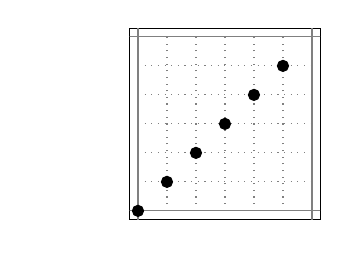
\begin{tikzpicture}
							\begin{axis}[
								plot box ratio = 1 1,
								xmin=-1/21,xmax=22/21,ymin=-1/21,ymax=22/21,
								font=\footnotesize,
								height=0.33\textwidth,
								width=0.33\textwidth,
								xticklabel = \empty,
								yticklabel = \empty,
								ytick style={draw=none},
								xtick style={draw=none},
								]
								\addplot[only marks,black,mark=*,mark size=2pt,mark options={solid}] coordinates {
									(0, 0) (1/6, 1/6) (1/3, 1/3) (1/2, 1/2) (2/3, 2/3) (5/6, 5/6)
								};
								\addplot[gray,mark options={solid}] coordinates {
									(0, -0.05) (0, 1.05)
								};
								\addplot[gray,mark options={solid}] coordinates {
									(1.0, -0.05) (1.0, 1.05)
								};
								\addplot[gray,mark options={solid}] coordinates {
									(-0.05, 0) (1.05, 0)
								};
								\addplot[gray,mark options={solid}] coordinates {
									(-0.05, 1.0) (1.05, 1.0)
								};
								\addplot[gray,mark options={solid}, dotted] coordinates {
									(0, 1/6) (1, 1/6)
								};
								\addplot[gray,mark options={solid}, dotted] coordinates {
									(0, 1/3) (1, 1/3)
								};
								\addplot[gray,mark options={solid}, dotted] coordinates {
									(0, 1/2) (1, 1/2)
								};
								\addplot[gray,mark options={solid}, dotted] coordinates {
									(1/6, 0) (1/6, 1)
								};
								\addplot[gray,mark options={solid}, dotted] coordinates {
									(1/3, 0) (1/3, 1)
								};
								\addplot[gray,mark options={solid}, dotted] coordinates {
									(1/2, 0) (1/2, 1)
								};
								\addplot[gray,mark options={solid}, dotted] coordinates {
									(0, 2/3) (1, 2/3)
								};
								\addplot[gray,mark options={solid}, dotted] coordinates {
									(0, 5/6) (1, 5/6)
								};
								\addplot[gray,mark options={solid}, dotted] coordinates {
									(2/3, 0) (2/3, 1)
								};
								\addplot[gray,mark options={solid}, dotted] coordinates {
									(5/6, 0) (5/6, 1)
								};
							\end{axis}
						\end{tikzpicture}
                        %2
                        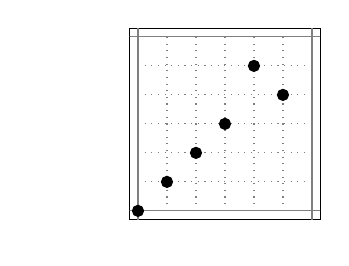
\begin{tikzpicture}
							\begin{axis}[
								plot box ratio = 1 1,
								xmin=-1/21,xmax=22/21,ymin=-1/21,ymax=22/21,
								font=\footnotesize,
								height=0.33\textwidth,
								width=0.33\textwidth,
								xticklabel = \empty,
								yticklabel = \empty,
								ytick style={draw=none},
								xtick style={draw=none},
								]
								\addplot[only marks,black,mark=*,mark size=2pt,mark options={solid}] coordinates {
									(0, 0) (1/6, 1/6) (1/3, 1/3) (1/2, 1/2) (2/3, 5/6) (5/6, 2/3)
								};
								\addplot[gray,mark options={solid}] coordinates {
									(0, -0.05) (0, 1.05)
								};
								\addplot[gray,mark options={solid}] coordinates {
									(1.0, -0.05) (1.0, 1.05)
								};
								\addplot[gray,mark options={solid}] coordinates {
									(-0.05, 0) (1.05, 0)
								};
								\addplot[gray,mark options={solid}] coordinates {
									(-0.05, 1.0) (1.05, 1.0)
								};
								\addplot[gray,mark options={solid}, dotted] coordinates {
									(0, 1/6) (1, 1/6)
								};
								\addplot[gray,mark options={solid}, dotted] coordinates {
									(0, 1/3) (1, 1/3)
								};
								\addplot[gray,mark options={solid}, dotted] coordinates {
									(0, 1/2) (1, 1/2)
								};
								\addplot[gray,mark options={solid}, dotted] coordinates {
									(1/6, 0) (1/6, 1)
								};
								\addplot[gray,mark options={solid}, dotted] coordinates {
									(1/3, 0) (1/3, 1)
								};
								\addplot[gray,mark options={solid}, dotted] coordinates {
									(1/2, 0) (1/2, 1)
								};
								\addplot[gray,mark options={solid}, dotted] coordinates {
									(0, 2/3) (1, 2/3)
								};
								\addplot[gray,mark options={solid}, dotted] coordinates {
									(0, 5/6) (1, 5/6)
								};
								\addplot[gray,mark options={solid}, dotted] coordinates {
									(2/3, 0) (2/3, 1)
								};
								\addplot[gray,mark options={solid}, dotted] coordinates {
									(5/6, 0) (5/6, 1)
								};
							\end{axis}
						\end{tikzpicture}
                        %3
						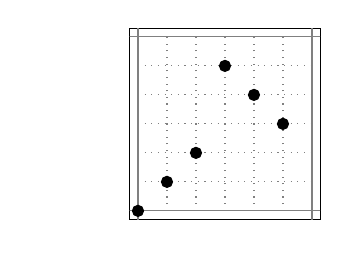
\begin{tikzpicture}
							\begin{axis}[
								plot box ratio = 1 1,
								xmin=-1/21,xmax=22/21,ymin=-1/21,ymax=22/21,
								font=\footnotesize,
								height=0.33\textwidth,
								width=0.33\textwidth,
								xticklabel = \empty,
								yticklabel = \empty,
								ytick style={draw=none},
								xtick style={draw=none},
								]
								\addplot[only marks,black,mark=*,mark size=2pt,mark options={solid}] coordinates {
									(0, 0) (1/6, 1/6) (1/3, 1/3) (1/2, 5/6) (2/3, 2/3) (5/6, 1/2)
								};
								\addplot[gray,mark options={solid}] coordinates {
									(0, -0.05) (0, 1.05)
								};
								\addplot[gray,mark options={solid}] coordinates {
									(1.0, -0.05) (1.0, 1.05)
								};
								\addplot[gray,mark options={solid}] coordinates {
									(-0.05, 0) (1.05, 0)
								};
								\addplot[gray,mark options={solid}] coordinates {
									(-0.05, 1.0) (1.05, 1.0)
								};
								\addplot[gray,mark options={solid}, dotted] coordinates {
									(0, 1/6) (1, 1/6)
								};
								\addplot[gray,mark options={solid}, dotted] coordinates {
									(0, 1/3) (1, 1/3)
								};
								\addplot[gray,mark options={solid}, dotted] coordinates {
									(0, 1/2) (1, 1/2)
								};
								\addplot[gray,mark options={solid}, dotted] coordinates {
									(1/6, 0) (1/6, 1)
								};
								\addplot[gray,mark options={solid}, dotted] coordinates {
									(1/3, 0) (1/3, 1)
								};
								\addplot[gray,mark options={solid}, dotted] coordinates {
									(1/2, 0) (1/2, 1)
								};
								\addplot[gray,mark options={solid}, dotted] coordinates {
									(0, 2/3) (1, 2/3)
								};
								\addplot[gray,mark options={solid}, dotted] coordinates {
									(0, 5/6) (1, 5/6)
								};
								\addplot[gray,mark options={solid}, dotted] coordinates {
									(2/3, 0) (2/3, 1)
								};
								\addplot[gray,mark options={solid}, dotted] coordinates {
									(5/6, 0) (5/6, 1)
								};
							\end{axis}
						\end{tikzpicture}

%\hspace{-1.1cm}
                        \hspace{-0.85cm} 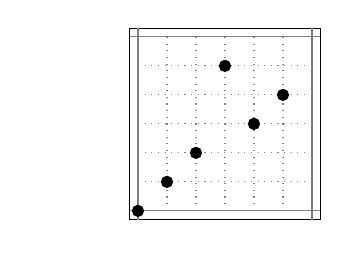
\begin{tikzpicture}
							\begin{axis}[
								plot box ratio = 1 1,
								xmin=-1/21,xmax=22/21,ymin=-1/21,ymax=22/21,
								font=\footnotesize,
								height=0.33\textwidth,
								width=0.33\textwidth,
								xticklabel = \empty,
								yticklabel = \empty,
								ytick style={draw=none},
								xtick style={draw=none},
								]
								\addplot[only marks,black,mark=*,mark size=2pt,mark options={solid}] coordinates {
									(0, 0) (1/6, 1/6) (1/3, 1/3) (1/2, 5/6) (2/3, 1/2) (5/6, 2/3)
								};
								\addplot[gray,mark options={solid}] coordinates {
									(0, -0.05) (0, 1.05)
								};
								\addplot[gray,mark options={solid}] coordinates {
									(1.0, -0.05) (1.0, 1.05)
								};
								\addplot[gray,mark options={solid}] coordinates {
									(-0.05, 0) (1.05, 0)
								};
								\addplot[gray,mark options={solid}] coordinates {
									(-0.05, 1.0) (1.05, 1.0)
								};
								\addplot[gray,mark options={solid}, dotted] coordinates {
									(0, 1/6) (1, 1/6)
								};
								\addplot[gray,mark options={solid}, dotted] coordinates {
									(0, 1/3) (1, 1/3)
								};
								\addplot[gray,mark options={solid}, dotted] coordinates {
									(0, 1/2) (1, 1/2)
								};
								\addplot[gray,mark options={solid}, dotted] coordinates {
									(1/6, 0) (1/6, 1)
								};
								\addplot[gray,mark options={solid}, dotted] coordinates {
									(1/3, 0) (1/3, 1)
								};
								\addplot[gray,mark options={solid}, dotted] coordinates {
									(1/2, 0) (1/2, 1)
								};
								\addplot[gray,mark options={solid}, dotted] coordinates {
									(0, 2/3) (1, 2/3)
								};
								\addplot[gray,mark options={solid}, dotted] coordinates {
									(0, 5/6) (1, 5/6)
								};
								\addplot[gray,mark options={solid}, dotted] coordinates {
									(2/3, 0) (2/3, 1)
								};
								\addplot[gray,mark options={solid}, dotted] coordinates {
									(5/6, 0) (5/6, 1)
								};
							\end{axis}
						\end{tikzpicture}
                        %5
                        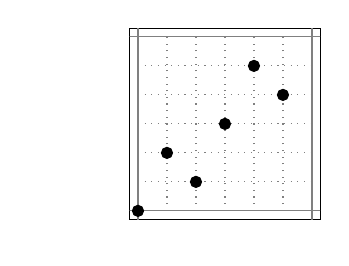
\begin{tikzpicture}
							\begin{axis}[
								plot box ratio = 1 1,
								xmin=-1/21,xmax=22/21,ymin=-1/21,ymax=22/21,
								font=\footnotesize,
								height=0.33\textwidth,
								width=0.33\textwidth,
								xticklabel = \empty,
								yticklabel = \empty,
								ytick style={draw=none},
								xtick style={draw=none},
								]
								\addplot[only marks,black,mark=*,mark size=2pt,mark options={solid}] coordinates {
									(0, 0) (1/6, 1/3) (1/3, 1/6) (1/2, 1/2) (2/3, 5/6) (5/6, 2/3)
								};
								\addplot[gray,mark options={solid}] coordinates {
									(0, -0.05) (0, 1.05)
								};
								\addplot[gray,mark options={solid}] coordinates {
									(1.0, -0.05) (1.0, 1.05)
								};
								\addplot[gray,mark options={solid}] coordinates {
									(-0.05, 0) (1.05, 0)
								};
								\addplot[gray,mark options={solid}] coordinates {
									(-0.05, 1.0) (1.05, 1.0)
								};
								\addplot[gray,mark options={solid}, dotted] coordinates {
									(0, 1/6) (1, 1/6)
								};
								\addplot[gray,mark options={solid}, dotted] coordinates {
									(0, 1/3) (1, 1/3)
								};
								\addplot[gray,mark options={solid}, dotted] coordinates {
									(0, 1/2) (1, 1/2)
								};
								\addplot[gray,mark options={solid}, dotted] coordinates {
									(1/6, 0) (1/6, 1)
								};
								\addplot[gray,mark options={solid}, dotted] coordinates {
									(1/3, 0) (1/3, 1)
								};
								\addplot[gray,mark options={solid}, dotted] coordinates {
									(1/2, 0) (1/2, 1)
								};
								\addplot[gray,mark options={solid}, dotted] coordinates {
									(0, 2/3) (1, 2/3)
								};
								\addplot[gray,mark options={solid}, dotted] coordinates {
									(0, 5/6) (1, 5/6)
								};
								\addplot[gray,mark options={solid}, dotted] coordinates {
									(2/3, 0) (2/3, 1)
								};
								\addplot[gray,mark options={solid}, dotted] coordinates {
									(5/6, 0) (5/6, 1)
								};
							\end{axis}
						\end{tikzpicture}
                        %6
                        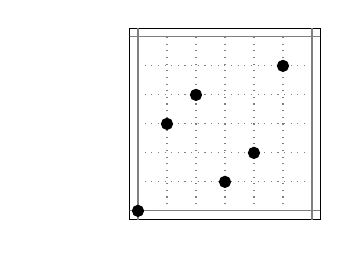
\begin{tikzpicture}
							\begin{axis}[
								plot box ratio = 1 1,
								xmin=-1/21,xmax=22/21,ymin=-1/21,ymax=22/21,
								font=\footnotesize,
								height=0.33\textwidth,
								width=0.33\textwidth,
								xticklabel = \empty,
								yticklabel = \empty,
								ytick style={draw=none},
								xtick style={draw=none},
								]
								\addplot[only marks,black,mark=*,mark size=2pt,mark options={solid}] coordinates {
									(0, 0) (1/6, 1/2) (1/3, 2/3) (1/2, 1/6) (2/3, 1/3) (5/6, 5/6)
								};
								\addplot[gray,mark options={solid}] coordinates {
									(0, -0.05) (0, 1.05)
								};
								\addplot[gray,mark options={solid}] coordinates {
									(1.0, -0.05) (1.0, 1.05)
								};
								\addplot[gray,mark options={solid}] coordinates {
									(-0.05, 0) (1.05, 0)
								};
								\addplot[gray,mark options={solid}] coordinates {
									(-0.05, 1.0) (1.05, 1.0)
								};
								\addplot[gray,mark options={solid}, dotted] coordinates {
									(0, 1/6) (1, 1/6)
								};
								\addplot[gray,mark options={solid}, dotted] coordinates {
									(0, 1/3) (1, 1/3)
								};
								\addplot[gray,mark options={solid}, dotted] coordinates {
									(0, 1/2) (1, 1/2)
								};
								\addplot[gray,mark options={solid}, dotted] coordinates {
									(1/6, 0) (1/6, 1)
								};
								\addplot[gray,mark options={solid}, dotted] coordinates {
									(1/3, 0) (1/3, 1)
								};
								\addplot[gray,mark options={solid}, dotted] coordinates {
									(1/2, 0) (1/2, 1)
								};
								\addplot[gray,mark options={solid}, dotted] coordinates {
									(0, 2/3) (1, 2/3)
								};
								\addplot[gray,mark options={solid}, dotted] coordinates {
									(0, 5/6) (1, 5/6)
								};
								\addplot[gray,mark options={solid}, dotted] coordinates {
									(2/3, 0) (2/3, 1)
								};
								\addplot[gray,mark options={solid}, dotted] coordinates {
									(5/6, 0) (5/6, 1)
								};
							\end{axis}
						\end{tikzpicture}


                        \hspace{-0.85cm} 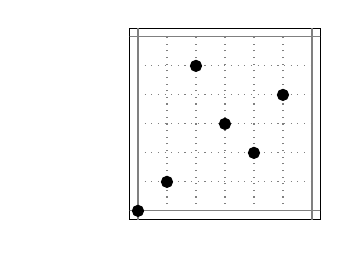
\begin{tikzpicture}
							\begin{axis}[
								plot box ratio = 1 1,
								xmin=-1/21,xmax=22/21,ymin=-1/21,ymax=22/21,
								font=\footnotesize,
								height=0.33\textwidth,
								width=0.33\textwidth,
								xticklabel = \empty,
								yticklabel = \empty,
								ytick style={draw=none},
								xtick style={draw=none},
								]
								\addplot[only marks,black,mark=*,mark size=2pt,mark options={solid}] coordinates {
									(0, 0) (1/6, 1/6) (1/3, 5/6) (1/2, 1/2) (2/3, 1/3) (5/6, 2/3)
								};
								\addplot[gray,mark options={solid}] coordinates {
									(0, -0.05) (0, 1.05)
								};
								\addplot[gray,mark options={solid}] coordinates {
									(1.0, -0.05) (1.0, 1.05)
								};
								\addplot[gray,mark options={solid}] coordinates {
									(-0.05, 0) (1.05, 0)
								};
								\addplot[gray,mark options={solid}] coordinates {
									(-0.05, 1.0) (1.05, 1.0)
								};
								\addplot[gray,mark options={solid}, dotted] coordinates {
									(0, 1/6) (1, 1/6)
								};
								\addplot[gray,mark options={solid}, dotted] coordinates {
									(0, 1/3) (1, 1/3)
								};
								\addplot[gray,mark options={solid}, dotted] coordinates {
									(0, 1/2) (1, 1/2)
								};
								\addplot[gray,mark options={solid}, dotted] coordinates {
									(1/6, 0) (1/6, 1)
								};
								\addplot[gray,mark options={solid}, dotted] coordinates {
									(1/3, 0) (1/3, 1)
								};
								\addplot[gray,mark options={solid}, dotted] coordinates {
									(1/2, 0) (1/2, 1)
								};
								\addplot[gray,mark options={solid}, dotted] coordinates {
									(0, 2/3) (1, 2/3)
								};
								\addplot[gray,mark options={solid}, dotted] coordinates {
									(0, 5/6) (1, 5/6)
								};
								\addplot[gray,mark options={solid}, dotted] coordinates {
									(2/3, 0) (2/3, 1)
								};
								\addplot[gray,mark options={solid}, dotted] coordinates {
									(5/6, 0) (5/6, 1)
								};
							\end{axis}
						\end{tikzpicture}
                        %8
                        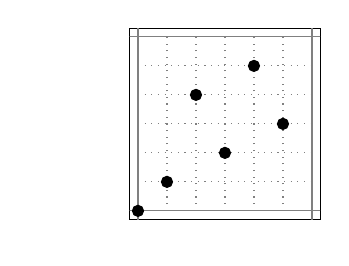
\begin{tikzpicture}
							\begin{axis}[
								plot box ratio = 1 1,
								xmin=-1/21,xmax=22/21,ymin=-1/21,ymax=22/21,
								font=\footnotesize,
								height=0.33\textwidth,
								width=0.33\textwidth,
								xticklabel = \empty,
								yticklabel = \empty,
								ytick style={draw=none},
								xtick style={draw=none},
								]
								\addplot[only marks,black,mark=*,mark size=2pt,mark options={solid}] coordinates {
									(0, 0) (1/6, 1/6) (1/3, 2/3) (1/2, 1/3) (2/3, 5/6) (5/6, 1/2)
								};
								\addplot[gray,mark options={solid}] coordinates {
									(0, -0.05) (0, 1.05)
								};
								\addplot[gray,mark options={solid}] coordinates {
									(1.0, -0.05) (1.0, 1.05)
								};
								\addplot[gray,mark options={solid}] coordinates {
									(-0.05, 0) (1.05, 0)
								};
								\addplot[gray,mark options={solid}] coordinates {
									(-0.05, 1.0) (1.05, 1.0)
								};
								\addplot[gray,mark options={solid}, dotted] coordinates {
									(0, 1/6) (1, 1/6)
								};
								\addplot[gray,mark options={solid}, dotted] coordinates {
									(0, 1/3) (1, 1/3)
								};
								\addplot[gray,mark options={solid}, dotted] coordinates {
									(0, 1/2) (1, 1/2)
								};
								\addplot[gray,mark options={solid}, dotted] coordinates {
									(1/6, 0) (1/6, 1)
								};
								\addplot[gray,mark options={solid}, dotted] coordinates {
									(1/3, 0) (1/3, 1)
								};
								\addplot[gray,mark options={solid}, dotted] coordinates {
									(1/2, 0) (1/2, 1)
								};
								\addplot[gray,mark options={solid}, dotted] coordinates {
									(0, 2/3) (1, 2/3)
								};
								\addplot[gray,mark options={solid}, dotted] coordinates {
									(0, 5/6) (1, 5/6)
								};
								\addplot[gray,mark options={solid}, dotted] coordinates {
									(2/3, 0) (2/3, 1)
								};
								\addplot[gray,mark options={solid}, dotted] coordinates {
									(5/6, 0) (5/6, 1)
								};
							\end{axis}
						\end{tikzpicture}
                        %9
                        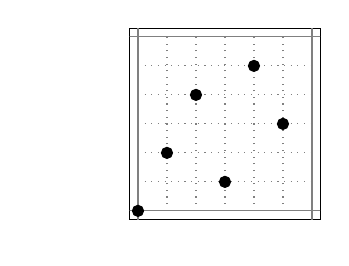
\begin{tikzpicture}
							\begin{axis}[
								plot box ratio = 1 1,
								xmin=-1/21,xmax=22/21,ymin=-1/21,ymax=22/21,
								font=\footnotesize,
								height=0.33\textwidth,
								width=0.33\textwidth,
								xticklabel = \empty,
								yticklabel = \empty,
								ytick style={draw=none},
								xtick style={draw=none},
								]
								\addplot[only marks,black,mark=*,mark size=2pt,mark options={solid}] coordinates {
									(0, 0) (1/6, 1/3) (1/3, 2/3) (1/2, 1/6) (2/3, 5/6) (5/6, 1/2)
								};
								\addplot[gray,mark options={solid}] coordinates {
									(0, -0.05) (0, 1.05)
								};
								\addplot[gray,mark options={solid}] coordinates {
									(1.0, -0.05) (1.0, 1.05)
								};
								\addplot[gray,mark options={solid}] coordinates {
									(-0.05, 0) (1.05, 0)
								};
								\addplot[gray,mark options={solid}] coordinates {
									(-0.05, 1.0) (1.05, 1.0)
								};
								\addplot[gray,mark options={solid}, dotted] coordinates {
									(0, 1/6) (1, 1/6)
								};
								\addplot[gray,mark options={solid}, dotted] coordinates {
									(0, 1/3) (1, 1/3)
								};
								\addplot[gray,mark options={solid}, dotted] coordinates {
									(0, 1/2) (1, 1/2)
								};
								\addplot[gray,mark options={solid}, dotted] coordinates {
									(1/6, 0) (1/6, 1)
								};
								\addplot[gray,mark options={solid}, dotted] coordinates {
									(1/3, 0) (1/3, 1)
								};
								\addplot[gray,mark options={solid}, dotted] coordinates {
									(1/2, 0) (1/2, 1)
								};
								\addplot[gray,mark options={solid}, dotted] coordinates {
									(0, 2/3) (1, 2/3)
								};
								\addplot[gray,mark options={solid}, dotted] coordinates {
									(0, 5/6) (1, 5/6)
								};
								\addplot[gray,mark options={solid}, dotted] coordinates {
									(2/3, 0) (2/3, 1)
								};
								\addplot[gray,mark options={solid}, dotted] coordinates {
									(5/6, 0) (5/6, 1)
								};
							\end{axis}
						\end{tikzpicture}
\caption{The $9$ possible distinct permutation sets in approximate order of decreasing energy, with the best possible configuration last.}
\label{fig:six_configs}
\end{figure}

\begin{proof}

Just as in the $N=4$ case we note that since $f$ is logarithmically convex and differentiable, we can find a minimizer given a specific permutation type by finding a configuration of the permutation type that is stationary with respect to the energy $E_F$ in the $x$- and $y$-coordinates of every point. It is straightforward to calculate the $10$ partial derivatives with respect to the coordinates of $\bx^1=(x^1_1, x^1_2), \dots, \bx^5=(x_1^5, x_2^5)$. Setting these partial derivatives to $0$, one obtains condition \eqref{eq:n6_condition} for $X_a^{(6)}$.
%\textcolor{red}{We note that unlike in Proposition \ref{prop:n4}, our configuration has two equivalence classes of points under reflections, coordinate permutations and translations: the points $(a,1/2-a)$ and $(a+1/2,1-a)$, and the points $(0,0),(2a,1-2a),(1/2,1/2-2a),(1/2+2a,1/2)$. The configuration has rotational symmetry of order $4$ around points in the first equivalence class and so these are necessarily stable in the $x$- and $y$-coordinates.}\todo{I don't quite follow this argument}To determine that the  other points are stationary, we will consider perturbations in the $x$- and $y$-coordinates of just one of the points, and a direct calculation shows that both partial derivatives yield the same condition, precisely \eqref{eq:n6_condition}.
We use the same argument as in the proof of Proposition \ref{prop:n4} to claim that a minimizer exists, and that it is unique in the case that $f$ is strictly logarithmically convex. 
%We note our configuration has associated energy $$E_F(X_{ab}):=4f(a)f(b)+4f(a+b)f(b-a)+2f(2a)f(2b)+4f(1/2-a)f(1/2-b).$$ 
%\begin{align*}\partial_aE_{ab}(a=1/6,b=1/3)&=4f'(1/6)f(1/3)-4f'(1/6)f(1/2)\\&+4f'(1/3)f(2/3)-4f'(1/3)f(1/6)\\
%\partial_bE_{ab}(a=1/6,b=1/3)&=4f'(1/3)f(1/6)+4f'(1/6)f(1/2)\\&+4f'(2/3)f(1/3)-4f'(1/6)f(1/3).\end{align*}
%Since $f(2/3)=f(1/3),f'(2/3)=-f'(1/3)$, we note that $$\partial_bE_{ab}(a=1/6,b=1/3)=-\partial_aE_{ab}(a=1/6,b=1/3).$$
\end{proof}

Unlike  the case $N=4$,  condition \eqref{eq:n6_condition} can be conceivably satisfied by the permutation set $X^{(6)}_{1/6}$ and in this case the condition becomes $$f'(1/6)(f(1/3)-f(1/2))=f'(1/3)(f(1/6)-f(1/3)).$$
Nevertheless, for the majority of potentials this equality will not be satisfied and thus in general the energy minimizer for $N=6$ will not be a permutation set, see Figure \ref{fig:6_pts}.%\todo[inline]{Include the example $e^{|x-1/2|}$}

%\todo[inline]{N: These point sets make me wonder:

%The $4$- and $6$-point cases above can be reduced to a $1$-dimensional optimization problem for the parameter $a$. For all $a$, the distance distribution of the shifted point set $X_a$ essentially does not change structurally. Can one, for every permutation, determine the number of parameters to characterize the space of all point sets of the same permutation type and essentially the same distance distribution?

%Lattices are rigid, so their parameter space is $0$-dimensional (I guess?). The previous two examples seemingly yield a $1$-dimensional parameter space. Does the number of parameters correlate with the ``uniformity'' of the point set?}

%\section{Conclusion}

%Open questions: transposition algorithm? permutation statistics? universal optimality? why Fibonacci? (roughly) equispaced coordinates? deeper meaning relation extr vs per? other occurrences of tensor product energies? higher dimensions?

\begin{figure}[htp]
\hspace{-1cm}
						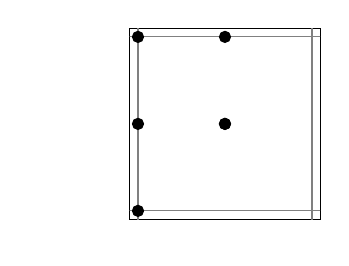
\begin{tikzpicture}
							\begin{axis}[
								plot box ratio = 1 1,
								xmin=-1/21,xmax=22/21,ymin=-1/21,ymax=22/21,
								font=\footnotesize,
								height=0.33\textwidth,
								width=0.33\textwidth,
								xticklabel = \empty,
								yticklabel = \empty,
								ytick style={draw=none},
								xtick style={draw=none},
								]
								\addplot[only marks,black,mark=*,mark size=2pt,mark options={solid}] coordinates {
									(0, 0) (0, 0.5) (0, 1) (0.5, 0.5) (0.5, 1) (0.5, 0.5)
								};
								\addplot[gray,mark options={solid}] coordinates {
									(0, -0.05) (0, 1.05)
								};
								\addplot[gray,mark options={solid}] coordinates {
									(1.0, -0.05) (1.0, 1.05)
								};
								\addplot[gray,mark options={solid}] coordinates {
									(-0.05, 0) (1.05, 0)
								};
								\addplot[gray,mark options={solid}] coordinates {
									(-0.05, 1.0) (1.05, 1.0)
								};
							\end{axis}
						\end{tikzpicture}
                        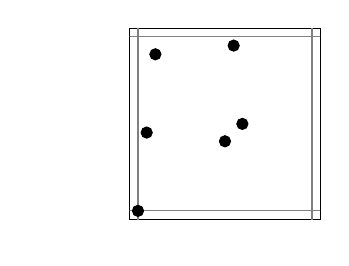
\begin{tikzpicture}
							\begin{axis}[
								plot box ratio = 1 1,
								xmin=-1/21,xmax=22/21,ymin=-1/21,ymax=22/21,
								font=\footnotesize,
								height=0.33\textwidth,
								width=0.33\textwidth,
								xticklabel = \empty,
								yticklabel = \empty,
								ytick style={draw=none},
								xtick style={draw=none},
								]
								\addplot[only marks,black,mark=*,mark size=2pt,mark options={solid}] coordinates {
									(0, 0) (0.05, 0.45) (0.1, 0.9) (0.5, 0.4) (0.55, 0.95) (0.6, 0.5)
								};
								\addplot[gray,mark options={solid}] coordinates {
									(0, -0.05) (0, 1.05)
								};
								\addplot[gray,mark options={solid}] coordinates {
									(1.0, -0.05) (1.0, 1.05)
								};
								\addplot[gray,mark options={solid}] coordinates {
									(-0.05, 0) (1.05, 0)
								};
								\addplot[gray,mark options={solid}] coordinates {
									(-0.05, 1.0) (1.05, 1.0)
								};
							\end{axis}
						\end{tikzpicture}
                        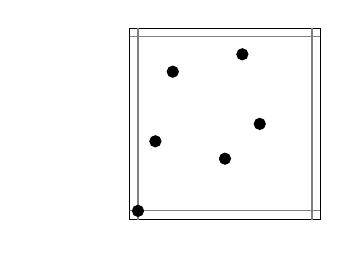
\begin{tikzpicture}
							\begin{axis}[
								plot box ratio = 1 1,
								xmin=-1/21,xmax=22/21,ymin=-1/21,ymax=22/21,
								font=\footnotesize,
								height=0.33\textwidth,
								width=0.33\textwidth,
								xticklabel = \empty,
								yticklabel = \empty,
								ytick style={draw=none},
								xtick style={draw=none},
								]
								\addplot[only marks,black,mark=*,mark size=2pt,mark options={solid}] coordinates {
									(0, 0) (0.1, 0.4) (0.2, 0.8) (0.5, 0.3) (0.6, 0.9) (0.7, 0.5)
								};
								\addplot[gray,mark options={solid}] coordinates {
									(0, -0.05) (0, 1.05)
								};
								\addplot[gray,mark options={solid}] coordinates {
									(1.0, -0.05) (1.0, 1.05)
								};
								\addplot[gray,mark options={solid}] coordinates {
									(-0.05, 0) (1.05, 0)
								};
								\addplot[gray,mark options={solid}] coordinates {
									(-0.05, 1.0) (1.05, 1.0)
								};
							\end{axis}
						\end{tikzpicture}

\hspace{-1cm}
                        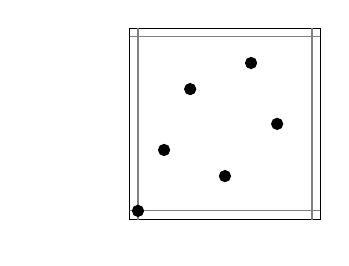
\begin{tikzpicture}
							\begin{axis}[
								plot box ratio = 1 1,
								xmin=-1/21,xmax=22/21,ymin=-1/21,ymax=22/21,
								font=\footnotesize,
								height=0.33\textwidth,
								width=0.33\textwidth,
								xticklabel = \empty,
								yticklabel = \empty,
								ytick style={draw=none},
								xtick style={draw=none},
								]
								\addplot[only marks,black,mark=*,mark size=2pt,mark options={solid}] coordinates {
									(0, 0) (0.15, 0.35) (0.3, 0.7) (0.5, 0.2) (0.65, 0.85) (0.8, 0.5)
								};
								\addplot[gray,mark options={solid}] coordinates {
									(0, -0.05) (0, 1.05)
								};
								\addplot[gray,mark options={solid}] coordinates {
									(1.0, -0.05) (1.0, 1.05)
								};
								\addplot[gray,mark options={solid}] coordinates {
									(-0.05, 0) (1.05, 0)
								};
								\addplot[gray,mark options={solid}] coordinates {
									(-0.05, 1.0) (1.05, 1.0)
								};
							\end{axis}
						\end{tikzpicture}
                        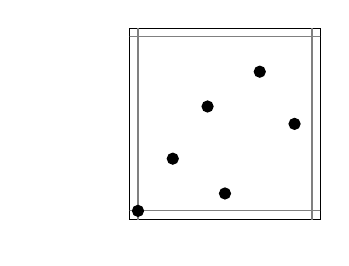
\begin{tikzpicture}
							\begin{axis}[
								plot box ratio = 1 1,
								xmin=-1/21,xmax=22/21,ymin=-1/21,ymax=22/21,
								font=\footnotesize,
								height=0.33\textwidth,
								width=0.33\textwidth,
								xticklabel = \empty,
								yticklabel = \empty,
								ytick style={draw=none},
								xtick style={draw=none},
								]
								\addplot[only marks,black,mark=*,mark size=2pt,mark options={solid}] coordinates {
									(0, 0) (0.2, 0.3) (0.4, 0.6) (0.5, 0.1) (0.7, 0.8) (0.9, 0.5)
								};
								\addplot[gray,mark options={solid}] coordinates {
									(0, -0.05) (0, 1.05)
								};
								\addplot[gray,mark options={solid}] coordinates {
									(1.0, -0.05) (1.0, 1.05)
								};
								\addplot[gray,mark options={solid}] coordinates {
									(-0.05, 0) (1.05, 0)
								};
								\addplot[gray,mark options={solid}] coordinates {
									(-0.05, 1.0) (1.05, 1.0)
								};
							\end{axis}
						\end{tikzpicture}
                        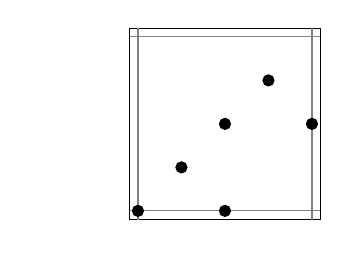
\begin{tikzpicture}
							\begin{axis}[
								plot box ratio = 1 1,
								xmin=-1/21,xmax=22/21,ymin=-1/21,ymax=22/21,
								font=\footnotesize,
								height=0.33\textwidth,
								width=0.33\textwidth,
								xticklabel = \empty,
								yticklabel = \empty,
								ytick style={draw=none},
								xtick style={draw=none},
								]
								\addplot[only marks,black,mark=*,mark size=2pt,mark options={solid}] coordinates {
									(0, 0) (0.25, 0.25) (0.5, 0.5) (0.5, 0) (0.75, 0.75) (1, 0.5)
								};
								\addplot[gray,mark options={solid}] coordinates {
									(0, -0.05) (0, 1.05)
								};
								\addplot[gray,mark options={solid}] coordinates {
									(1.0, -0.05) (1.0, 1.05)
								};
								\addplot[gray,mark options={solid}] coordinates {
									(-0.05, 0) (1.05, 0)
								};
								\addplot[gray,mark options={solid}] coordinates {
									(-0.05, 1.0) (1.05, 1.0)
								};
							\end{axis}
						\end{tikzpicture}
\caption{$X_a^{(6)}$ for $a \in \{0, 0.05, 0.1, 0.15, 0.2, 0.25\}$ (with the double points $(0.5, 0.5)$ and $(0, 0) \simeq (0, 1)$ for $a=0$). For the potential $f(t) = \frac12-t+t^2$ the minimizer is attained for $a=0.16375\dots$ solving $20a^3-15a^2+\frac{13}2a-\frac34=0$.}\label{fig:6_pts}
\end{figure}

\section*{Acknowledgment}

%\todo[inline]{grants etc.}

DB was supported by the Simons Travel Support for Mathematicians and the Fulbright-NAWI Graz Visiting Professor fellowship.   NN was supported by the ESF Plus Young Researchers Group ReSIDA-H2 (SAB, 10064931). We would also like to thank Alexey Glazyrin for fruitful discussions. 

\appendix

\section*{Appendix}

\section{A collection of potentials}\label{s.potentials}

In this section we  collect some potentials which are relevant in the context of tensor product energy. Natural examples arise from discrepancy theory, quasi-Monte Carlo integration and harmonic analysis. F%or theoretical considerations we 
We also give  other examples which might shed  light on optimal point configurations. %We only list some potentials here, for more details consult the cited references.\todo[inline]{We could maybe get rid of this last sentence.}

\paragraph{Quasi-Monte Carlo integration.} Let $s \in \bbN$ and let $a_{-1}, a_0, a_1, \dots,$ $a_s \geq 0$ be parameters with $a_s > 0$ and $a_{-1}+ a_0 > 0$. Let $H^s_\ba(\bbT)$ be the Sobolev space of periodic functions $f: \bbT \rightarrow \bbR$ such that $f^{(k)} \in L_2(\bbT)$ for all weak derivatives of order $k=0, 1, \dots, s$, equipped with the norm (which is a norm by the assumptions on the parameters $a_i$)
$$
\|f\|_{H^s_\ba(\bbT)}^2 \coloneqq a_{-1} \left(\int_\bbT f(x) \, \dx x\right)^2 + \sum_{k=0}^s a_k \int_\bbT f^{(k)}(x)^2 \, \dx x.
$$
This turns $H^s_\ba(\bbT)$ into a reproducing kernel Hilbert space with kernel given by
$$
K_\ba(x, y) = \sum_{m \in \bbZ} \frac{\exp(2\pi\iu m (x-y))}{a_{-1} \delta_{m, 0} + \sum_{k=0}^s a_k (2\pi m)^{2k}}.
$$
For $d$ dimensions we simply take a $d$-fold tensor product $H^s_\ba(\bbT^d) = H^s_\ba(\bbT) \otimes \dots \otimes H^s_\ba(\bbT)$, whose kernel can be given by
$$
K_\ba^d(\bx, \by) = \prod_{i=1}^d K_\ba(x_i, y_i).
$$
Spaces like these are sometimes also called \emph{Korobov spaces} \cite{Dic08, DSWW06, GL22, Kuo03}, although note that some authors use this term for different spaces \cite{DTU18, KNU25, Kor59}. For $X \sbse \bbT^d, \#X = N$ the worst case error of the quasi-Monte Carlo rule can be determined to be \cite{NW10}
$$
\sup_{\|f\|_{H^s_\ba(\bbT^d)} \leq 1} \left|\frac1N \sum_{\bx \in X} f(\bx) - \int_{\bbT^d} f(\bx) \, \dx\bx\right|^2 = -\frac1{(a_{-1} + a_0)^d} + \frac1{N^2} \sum_{\bx, \by \in X} K_\ba^d(\bx, \by).
$$
Minimizing the worst case error is thus equivalent to minimizing
$$
\sum_{\substack{\bx, \by \in X \\ \bx \neq \by}} K_\ba^d(\bx, \by),
$$
which, since the kernel is of the form $K_\ba^d(\bx, \by) = \prod_{i=1}^d f_\ba(x_i-y_i)$, can be interpreted as a tensor product energy. A particular example would be, for $p > 0$ a parameter, $a_{-1} = 1$, $a_{s} = p^{-1}$ and $a_0 = a_1 = \dots = a_{s-1} = 0$, for which the kernel is of the form
$$
K_\ba(x, y) = 1 + (-1)^{s-1} \frac{p}{(2s)!} B_{2s}(x-y),
$$
where $B_{2s}$ is a Bernoulli polynomial of degree $2s$, given by
\begin{align} \label{eq:Bernoulli_poly}
	B_{2s}(t) = - (2s)! \sum_{m \neq 0} \frac{\exp(2\pi\iu m t)}{(2\pi\iu m)^{2s}}.
\end{align}
The case of $s = 1$ and $p \in \{1, 6\}$ was considered in \cite{HO16}. More generally, these potentials were studied for $s=1$ in \cite{Nag25b}. Similar but slightly different potentials were considered in \cite{BD13b}.

\paragraph{(Smooth) Discrepancy.} Discrepancy quantifies how uniform a set $X \sbse \bbT^d$ is in a geometric way. We describe the definition here and show its relation to the quasi-Monte Carlo method. Let $s \in \bbN$ and for $x \in \bbR$ define the B-splines
$$
B_{0, 1}^1(x) \coloneqq \chi^{}_{[0, 1)}(x)
$$
and recursively
$$
B_{0, 1}^s(x) \coloneqq \int_{x-1}^x B_{0, 1}^{s-1}(u) \, \dx u = \int_0^1 B_{0, 1}^{s-1}(x-u) \, \dx u.
$$
Note that $\supp B_{0, 1}^s = [0, s]$. With $(x)_+ \coloneqq \max\{0, x\}$ we even have explicitly
$$
B_{0, 1}^s(x) = \frac{1}{(s-1)!} \sum_{k=0}^s (-1)^k {s \choose k} (x-k)_+^{s-1}.
$$
For $0 \leq \alpha < 1$ and $0 < \delta \leq 1$ set
$$
B_{\alpha, \delta}^s(x) \coloneqq B_{0, 1}^s\left(\frac{x-\alpha}\delta\right) = \delta^{-1} \int_0^\delta B_{\alpha, \delta}^{s-1}(x-u) \, \dx u
$$
with $\supp B_{\alpha, \delta}^s = [\alpha, \alpha + s \delta]$. For $x \in [0, 1) \simeq \bbT$ introduce the periodization
$$
\tilde B_{\alpha, \delta}^s(x) \coloneqq \sum_{k \in \bbZ} B_{\alpha, \delta}^s(k+x) = \delta^{-1} \int_0^\delta \tilde B_{\alpha, \delta}^{s-1}(x-u) \, \dx u,
$$
where $x-u \in \bbT$ with wrap-around on the torus. Finally, let
\begin{align} \label{eq:phi_recursive}
	\varphi_{\alpha, \delta}^s(x) \coloneqq \delta^{s-1} \tilde B_{\alpha, \delta}^s(x) = \int_0^\delta \varphi_{\alpha, \delta}^{s-1}(x-u) \, \dx u.
\end{align}
It is easy to verify that
\begin{itemize}
	\item $\varphi_{\alpha, \delta}^1(x) = \chi^{}_{[\alpha, \{\alpha + \delta\})}(x)$ in the sense of periodic intervals \cite{HKP21}, where $\{\cdot\}$ denotes the fractional part,
	
	\item $\varphi_{\alpha, 1}^s(x) \equiv 1$ and
	
	\item $\int_0^1 \varphi_{\alpha, \delta}^s(x) \, \dx x = \delta^s$.
\end{itemize}
Let us collect some facts about these functions $\varphi_{\alpha, \delta}^s$.
\begin{lem} \label{lem:spline_properties}
	We have the Fourier representation (with convergence in $L_2$)
	\begin{align} \label{eq:spline_fourier}
		\varphi_{\alpha, \delta}^s(x) = \delta^s + \sum_{m \neq 0} \left(\frac{1-\exp(-2\pi\iu m \delta)}{2\pi\iu m}\right)^s \exp(2\pi\iu m (x-\alpha)).
	\end{align}
	Furthermore, for all $x, y \in [0, 1)$ it holds
	\begin{align} \label{eq:spline_inner_prod}
		\int_0^1 \int_0^1 \varphi_{\alpha, \delta}^s(x) \varphi_{\alpha, \delta}^s(y) \, \dx \delta \, \dx \alpha = \frac1{2s+1} + \frac{(-1)^{s-1}}{(s!)^2} B_{2s}(|x-y|).
	\end{align}
\end{lem}
\begin{proof}
	We prove \eqref{eq:spline_fourier} via induction on $s$. By periodicity we may assume $\alpha = 0$. For $s = 1$ we have $\varphi_{0, \delta}^1(x) = \chi^{}_{[0, \delta)}(x)$ with Fourier coefficients
	$$
	\int_0^1 \varphi_{0, \delta}^1(x) \exp(-2\pi\iu m x) \, \dx x = \begin{cases}
		\delta, & m = 0, \\
		\frac{1-\exp(-2\pi\iu m \delta)}{2\pi\iu m}, & m \neq 0.
	\end{cases}
	$$
	Assuming the formula holds for $s-1$, we have (using periodicity)
	\begin{align*}
		& \int_0^1 \varphi_{0, \delta}^s(x) \exp(-2\pi\iu m x) \, \dx x = \int_0^\delta \int_0^1 \varphi_{0, \delta}^{s-1}(x-u) \exp(-2\pi\iu m x) \, \dx x \, \dx u \\
		= & \int_0^\delta \exp(-2\pi\iu m u) \, \dx u \int_0^1 \varphi_{0, \delta}^{s-1}(x) \exp(-2\pi\iu m x) \, \dx x \\
		= & \begin{cases}
			\delta^s, & m = 0, \\
			\left(\frac{1-\exp(-2\pi\iu m \delta)}{2\pi\iu m}\right)^s, & m \neq 0.
		\end{cases}
	\end{align*}
	This shows \eqref{eq:spline_fourier}. We use this Fourier representation to show the second formula \eqref{eq:spline_inner_prod}. Indeed, we can then write
	\begin{align*}
		& \int_0^1 \int_0^1 \varphi_{\alpha, \delta}^s(x) \varphi_{\alpha, \delta}^s(y) \, \dx \delta \, \dx \alpha \\
		= & \frac1{2s+1} + \sum_{m \neq 0} \left( \int_0^1 \left|\frac{1-\exp(-2\pi\iu m \delta)}{2\pi\iu m}\right|^{2s} \, \dx \delta\right) \exp(2\pi\iu m (x-y)).
	\end{align*}
	Since for $t \in \bbR$ it holds
	$$
	|1- \exp(-\iu t)|^{2} = -\exp(-\iu t) (1-\exp(\iu t))^2,
	$$
	for $t = 2\pi m \delta$ we have
	\begin{align*}
		\int_0^1 |1- \exp(-2\pi\iu m \delta)|^{2s} \, \dx \delta & = (-1)^s \int_0^1 \exp(-2\pi\iu s m \delta) (1-\exp(2\pi\iu m \delta))^{2s} \, \dx \delta \\
		& = \sum_{k=0}^{2s} (-1)^{s+k} {2s \choose k} \int_0^1 \exp(2\pi\iu (k-s) m \delta) \, \dx \delta \\
		& = {2s \choose s}.
	\end{align*}
	This finally leads to the desired result (using \eqref{eq:Bernoulli_poly})
	\begin{align*}
		\int_0^1 \int_0^1 \varphi_{\alpha, \delta}^s(x) \varphi_{\alpha, \delta}^s(y) \, \dx \delta \, \dx \alpha & = \frac1{2s+1} + {2s \choose s} \sum_{m \neq 0} \frac{\exp(2\pi\iu m (x-y))}{(2\pi m)^{2s}} \\
		& = \frac1{2s+1} + \frac{(-1)^{s-1}}{(s!)^2} B_{2s}(|x-y|).
	\end{align*}
\end{proof}
%\begin{rem*}
%	It would be interesting to see if it is possible to show \eqref{eq:spline_inner_prod} more directly without using the Fourier expansion \eqref{eq:spline_fourier}, for example using the recursive definition of $\varphi_{\alpha, \delta}^s$ \eqref{eq:phi_recursive} together with some convolution identity for Bernoulli polynomials []. 
%\end{rem*}
The \emph{$s$-smooth periodic $L_2$-discrepancy} of a point set $X \sbse \bbT^d, \#X = N$ will be defined as
$$
L_{2, s}^{\text{per}}(X)^2 \coloneqq \int_{[0, 1)^d} \int_{(0, 1]^d} \left|\frac1N \sum_{\bx \in X} \prod_{i=1}^d \varphi_{\alpha_i, \delta_i}^s(x_i) - \int_{\bbT^d}\prod_{i=1}^d \varphi_{\alpha_i, \delta_i}^s(x_i) \, \dx \bx \right|^2 \, \dx \underline{\delta} \, \dx \underline{\alpha},
$$
where $\underline{\alpha} = (\alpha_1, \dots, \alpha_d)$ and $\underline{\delta} = (\delta_1, \dots, \delta_d)$. From Lemma \ref{lem:spline_properties} we conclude the following \emph{Warnock-type formula} for periodic discrepancy (the case for $s=1$ already appearing in \cite{HKP21, HO16}).
\begin{thm} \label{thm:smooth_discr}
	It holds
	\begin{align*}
		& L_{2, s}^{\text{per}}(X)^2 \\
		= & -\frac1{(2s+1)^d} + \frac1{N^2} \sum_{\bx, \by \in X} \prod_{i=1}^d \left(\frac1{2s+1} + \frac{(-1)^{s-1}}{(s!)^2} B_{2s}(|x_i-y_i|)\right).
	\end{align*}
\end{thm}
While the general equivalence of QMC and (smooth) discrepancy is well-known \cite{Tem19}, this explicit formula does not seem to have appeared in the literature so far. Comparing with $K_\ba^d$ from the previous part, we see that this is equivalent to the QMC worst case error over the space $H_\ba^s(\bbT^d)$ with parameters
$$
a_{-1} = 2s+1, a_0 = a_1 = \dots = a_{s-1} = 0, a_s = {2s \choose s}^{-1}.
$$

\paragraph{Diaphony.} Diaphony \cite{Lev95, Zin76} of $X \sbse \bbT^d, \#X = N$ is a quantity given by (without the square root)
$$
\sum_{\bm \in \bbZ} \left|\frac1N \sum_{\bx \in X} \exp(2\pi\iu \bm^\top \bx)\right|^2 \prod_{i=1}^d \begin{cases}
	1, & m_i = 0, \\
	\frac1{2\pi m_i}, & m_i \neq 0.
\end{cases}
$$
This is turns out to be the worst case error for the quasi-Monte Carlo rule over the space $H^1_\ba(\bbT^d)$ with parameters $a_{-1}=1, a_0 = 0, a_{1} = 1$.

\paragraph{Tensorized Poisson kernel.} The \emph{Poisson kernel} with parameter $r \in (0, 1)$ is given by
$$
P_r(t)= \sum_{m \neq 0} r^{|m|} \exp(2\pi\iu m t) = \frac{1-r^2}{1 - 2 r \cos(2\pi t) + r^2}
$$
for $t \in \bbT$. Tensorization leads to the kernel
$$
K^d_{P_r}(\bx, \by) \coloneqq \prod_{i=1}^d P_r(x_i-y_i),
$$
For fixed $r$ this can be seen as a kernel over a Sobolev space of infinite dominating mixed smoothness (with certain exponential decay of the Fourier coefficients).

\paragraph{Logarithmically convex potentials.} We finish by mentioning some logarithmically convex potentials. Here $k$ can be seen as a shape parameter and $c$ is a parameter that controls the logarithmic convexity for a certain range.
\begin{itemize}
	\item Polynomial potential
	$$
	f(t) = 1 + c\left(t^k + (1-t)^k\right), \quad k > 1, 0<c \leq k-1
	$$
	
	\item Another polynomial potential
	$$
	f(t) = 1 + c \left|2t-1\right|^k, \quad k > 1, 0<c \leq k-1
	$$
	
	\item Potential via the entropy function
	$$
	f(t) = 1 + c\left(t \ln t + (1-t) \ln (1-t)\right), \quad 0 < c \leq c_0 = 1.23325675\dots
	$$
	
	\item Ellipse potential
	$$
	f(t) = 1 - c \sqrt{t(1-t)}, \quad 0 < c \leq (3/2)^{3/2} = 1.8371173\dots
	$$
\end{itemize}

%\todo[inline]{For the entropy potential, one could probably write $c_0$ as a solution to some transcendental equation, but not sure if that would be worth it.}

\bibliographystyle{plain}
\bibliography{refs}

\end{document}






























\subsection{Main questions}

\todo[inline]{N: Incorporate questions naturally into the text, e.g. ``numerical evidence suggest the optimality of Fibonacci lattices etc.?}

As the discussion above in dimensions $d=1$ and $d=2$ indicates, permutation sets seem to be a natural choice for minimizers of tensor product energies $E_F$. This naturally leads to the following question:

\begin{q}
    Which conditions on the potential $f$ guarantee that the minimizers of the tensor product energy \eqref{e.energy} are permutation/Latin hypercube sets?
\end{q}

%\begin{center}
%    {\it  Which conditions on the potential $f$ guarantee that the minimizers of \\ the tensor product energy \eqref{e.energy} are permutation/Latin hypercube sets?} 
%\end{center}

This question admits a variety of versions and interpretations: e.g., when does this hold for all $N$, for specific values of $N$, or for all $N$ large enough?  Is there uniqueness? As the results in \cite{} indicate, we can only hope to get permutation sets as minimizers if the point set itself fulfills certain symmetry or regularity conditions. It is thus of interest to formulate the following variant of the above question:

\begin{q}
    When are global minimizers permutation/Latin hypercube sets for $N$-point sets restricted to the $N^d$-grid? If we consider general point sets $X \sbse \bbT^d$, can we guarantee that the coordinate projections of minimizers are roughly equispaced in a quantitative way?
\end{q}

%\begin{center}
%    {\it  When are global minimizers permutation/Latin hypercube sets for \\ $N$-point sets restricted to the $N^d$-grid? If we consider general point \\ sets $X \sbse \bbT^d$, can we guarantee that the coordinate projections of \\ minimizers are roughly equispaced in a quantitative way?} 
%\end{center}

These questions are motivated from an algorithmic point of view: can one find optimal point sets by first optimizing the permutation type among point sets living in the $(N \times N)$-grid and then doing fine adjustments via, for example, gradient descent?

In a more concrete direction, we ask the following:

\begin{q}
    If the potential $f$ is decreasing and log-convex in $(0, 1/2)$, and $N = F_j$ is a Fibonacci number, is the $N$-point Fibonacci lattice the global minimizer of $E_F(X)$ among all $N$-point configurations in $\bbT^2$?
\end{q}

%\begin{center}
%    \textit{If the potential $f$ is decreasing and log-convex in $(0, 1/2)$, and $N = F_j$ \\ 
%    is a Fibonacci number, is the $N$-point Fibonacci lattice the global \\ minimizer of $E_F(X)$ among all $N$-point configurations in $\bbT^2$?}
%\end{center}

An affirmative answer to this question would mirror known results on energy minimizers in the sphere. There, it is known that certain point configurations (so-called \emph{sharp configurations} as well as the vertices of the 600-cell) minimize the energy for a large class of potentials simultaneously, an effect known as \emph{universal optimality}. Such point sets are rare and need to posses extraordinary symmetry and regularity properties. We suspect that Fibonacci lattices are a new instance of this phenomenon. In particular, the $5$-point Fibonacci lattice
$$
\Phi_5 = \left\{\left(\frac05, \frac05\right), \left(\frac15, \frac35\right), \left(\frac25, \frac15\right), \left(\frac35, \frac45\right), \left(\frac45, \frac25\right)\right\}
$$
has certain properties resembling the ones of the sharp configurations on the sphere, namely
$$
\int_0^1 \int_0^1 \exp(2\pi\iu (mx+ny)) \, \dx x \, \dx y = \frac15 \sum_{(x, y) \in \Phi_5} \exp(2\pi\iu(mx+ny))
$$
for all $(m, n) \in \bbZ^2 \sm \{(m, n) \neq (0, 0): m+3n \equiv 0 \mod 5\}$ (exact discretization of the integral of Fourier functions on a large set of frequencies), as well as, recalling \eqref{eq:geod_dist},
$$
(\delta(x, \tilde x), \delta(y, \tilde y)) \in \left\{\left(\frac15, \frac25\right), \left(\frac25, \frac15\right)\right\}
$$
for all $(x, y), (\tilde x, \tilde y) \in \Phi_5, (x, y) \neq (\tilde x, \tilde y)$ (only few distances appearing in the point set). By the last property we have that
$$
E_F(\Phi_5) = 20 f\left(\frac15\right) f\left(\frac25\right),
$$
i.e. the interaction between two points is always the same. This will also be the key property for one of our main results Theorem \ref{thm:optimality} below.





\subsection{Main results}

While a complete resolution of the aforementioned questions appears to be out of reach at the moment, in the current  paper we present a series of results which provide strong evidence and important steps in this direction. Every section covers a certain class of potentials $f$ and properties of certain point sets with respect to this potential. The sections are ordered by how restrictive these conditions on $f$ are, with Section 2 covering the largest class of potentials. Below we summarize our main results.

In Section \ref{s.noequal} we prove under mild smoothness assumptions that if the local repulsion at small scales is sufficiently strong, in the sense that the potential $f: \bbT \rightarrow [0, \infty)$ if smooth except for a downwards opening kink at $0$, then any two points of the global (or even local) minimizer of the $N$-point energy have distinct $x_1$-coordinates (and, by symmetry, the same holds for the other coordinates). This holds for a wide range of kernels and might be construed as a first step towards demonstrating that permutation sets are (approximate) energy minimizers.

In Section \ref{s.1dist} we show that Latin hypercube sets with identical (up to a set of symmetries) interactions between its points, what we will call \emph{unique-distance sets}, are the minimizing configurations for potentials $f: \bbT \ra (0, \infty)$ with the property that minimizers in $\bbT$ of the potential $g = \log f$ are equispaced points. We completely classify lattices with this property. Special examples of such lattices are the $3$- and $5$-point Fibonacci lattice. We also determine some non-lattice point sets with this property. %Be careful with tense agreement! It would probably be best just to use present tense.

\TBC































\subsection{The $N=5$ case}

\todo[inline]{This subsection needs to be moved forward to/folded into section 3.}

\begin{lem}\label{lem:5perm}
    The Fibonacci lattice is a minimizing configuration among permutation sets of $5$ points.
\end{lem}

\begin{proof}
    We note that permutation sets in the $N=5$ case on $\mathbb{T}^2$ can contain only the distance vectors $(1/5,1/5),(1/5,2/5)$, and $(2/5,2/5)$. Since every point has two points that it differs by $1/5$ in the $x$-coordinate and two points that it differs by $2/5$ in the $x$-coordinate and we have the same result for the $y$-coordinate, we see that for a permutation set $X$, the expansion of the sum in $E_F(X)$ must contain $f(1/5)f(1/5)$ the same number of times as $f(2/5)f(2/5)$. Using $f(1/5)f(1/5)+f(2/5)f(2/5)\ge 2f(1/5)f(2/5)$ we conclude that for any permutation set $X$, $E_F(X)\ge 10f(1/5)f(2/5)$, which is the energy of the five point Fibonacci lattice. 
\end{proof}

We briefly discuss the case of energy minimization in dimension one mentioned in the introduction. For $N\in \mathbb N$ let us call an even $1$-periodic  function $N$-equispacing  if among all $N$-point configurations $\{x_0 ,\dots, x_{N-1}\}$ on $\mathbb T$ the energy $$ \sum_{\substack{i,j=1\\i\neq j}}^N f (x_i - x_j) $$ is minimized by equispaced points $x_j=j/N$. We recall some known conditions for the kernel to be equispacing:
\begin{itemize}
\item If $f$ is decreasing on $(0,1/2)$ and convex on $(0,1)$, then $f$ is equispacing for any $N\ge 0$ \cite{}.
\item Define the function $g: [-1,1]\rightarrow \mathbb R$ by $g (\cos (2\pi t)) = f(t)$. If $g$ is absolutely monotone (i.e. $g^{(n)} (t) \ge 0$ for all $t\in [-1,1)$ and $n\ge 0$), then $f$ is equispacing for any $N\ge 0$ \cite{}.
\item Let $N$ be fixed. Assume $f$ has absolutely convergent cosine series $\displaystyle{f(x) = \sum_{m=0}^\infty a_m \cos 2\pi mx}$ such that $a_m \ge 0 $ for all $m\ge0$ (i.e. $f$ is positive definite) and $a_m=0$ whenever $m>0$ is a multiple of $N$. Then $f$ is $N$-equispacing (this is a simple exercise).  
\end{itemize}
.
We are now ready to state the main result of the section.
\begin{thm}\label{thm.5u}
Assume that $f$ is an even, non-negative, $1$-periodic function, such that $\log f$ is $5$-equispacing. Then the five-point Fibonacci lattice minimizes the tensor product energy among all five-point configurations. 
\end{thm}

\begin{proof}
   Let us denote $h(x) = \log f(x)$. We can then estimate using Jensen's inequality
   \begin{align*}
       E_f(\mathbf{p}_0,\mathbf{p}_1,...,\mathbf{p}_4) &= \sum_{\substack{i,j =0\\ i\neq j }}^4 f(x_i - x_j) f (y_i -y_j)\\ 
       &= \sum_{\substack{i,j =0\\ i\neq j }}^4 \operatorname{exp} \big( h(x_i - x_j) + h( y_i -y_j) \big) \\
       & \ge 20 \operatorname{exp} \bigg( \frac{1}{20} \sum_{\substack{i,j =0\\ i\neq j }}^4 h(x_i - x_j) + \frac{1}{20} \sum_{\substack{i,j =0\\ i\neq j }}^4 h(y_i - y_j)\bigg).
   \end{align*}
   Since $h$ is $5$-equispacing, we know that the expressions in the exponent can be estimated as
   $$ \sum_{\substack{i,j =0\\ i\neq j }}^4 h(x_i - x_j) \ge \sum_{\substack{i,j =0\\ i\neq j }}^4 h\bigg(\frac{i - j}{5}\bigg) = 10 \big( h(1/5) + h(2/5)\big) .$$ We thus find that $$ E_f(\mathbf{p}_0,\mathbf{p}_1,...,\mathbf{p}_4) \ge 20 \operatorname{exp} \big( h(1/5) + h(2/5)\big) = 20 f(1/5)f(2/5). $$
   Finally, observe that the last expression is exactly the energy of the five-point Fibonacci lattice, since  interaction of every pair of points contributes precisely $f(1/5)f(2/5)$ to the energy. This finishes the proof. 
\end{proof}

This theorem can be applied  to all known  classes of $5$-equispacing functions listed above. The case of convex kernels presents special interest, so we formulate it as a corollary. 

\begin{cor}\label{c.N5}
    Assume that $f\ge0$ is $1$-periodic, even, decreasing  and log-convex on $(0,1/2)$ (equivalently, $F(x,y)=f(x)f(y)$ is convex). Then the five-point Fibonacci lattice minimizes the energy among all five-point configurations in $\mathbb T^2$. 
\end{cor}

\begin{rem*}
    We note that direct analogues of  Theorem \ref{thm.5u} and Corolary \ref{c.N5} could be formulated for $N=3$, since in this case lattices have the same property that each pair contributes the same amount to the energy. This would give an alternative proof of Corollary \ref{c.N3}. More generally, one can state such results for all lattices with this rather rare property. The characterization of such lattices is undertaken in Section \ref{s.1dist}.
\end{rem*}
